\vspace*{2cm}

{\bf \huge Part VI:}
\vspace{1cm}

{\Huge \bf And all that (eMoflon) jazz}
\vspace{1cm}

\genHeader

Welcome to the miscellaneous part of our eMoflon handbook. You can consider this
Part to be the `bonus' or appendix area of the entire handbook series. Here we have collected and documented a series of advanced topics related to our tool. These include some tips and tricks you may find helpful while using the tool with
Enterprise Architect (EA), a syntax reference table of our Moflon Specification Language (MOSL), and information about the protocol file generated with every
Triple Graph Grammar (TGG) transformation which we were never able to explain in Parts IV or V. This entire part is kept rather compact, intended to be used
mainly as a reference and consulted on demand.

Please note that if you're looking for instructions on how to properly export and import separate metamodels into the same project for work with TGG
transformations, please refer to Part IV, Section 2.2 (visual/EAP files) and 2.3 (textual/Eclipse projects), where we included detailed steps in the context of
an example.

If you feel anything is missing from this part, or if you have any other comments or suggestions about the handbook series and our tool, feel free to contact us
anytime at \href{mailto:contact@moflon.org}{contact@moflon.org}.

\newpage
\section{Grokking EA}
\visHeader

\vspace*{0.5cm}

\begin{quote} {\small Grok: ``\ldots to understand so thoroughly that the observer becomes a part of the observed.''\\
\hspace*{3.2cm} - Robert A. Heinlein, \emph{Stranger in a Strange land}}
\end{quote}

\vspace{0.5cm}

This section is a collection of a few of what we feel are the most important tips and tricks for working productively with EA. 
We truly believe that spending the time to learn and practice these is necessary for a pleasant modelling experience.

\vspace{0.5cm}

\section{Positioning elements}

Layout is always an important factor when using a visual language:
A well laid-out diagram is easiest to understand and, by centralizing important
elements or clustering related elements, you can actually impart additional information.

\begin{stepbystep}
\item To select a group of elements, either drag a selection box around the items or hold \texttt{Ctrl} and select each element
one-by-one.

\item In the top right corner of the last selected element, a small colon-styled symbol will appear (\Cref{ea:layout1}). Click on
this for a context list of different options you can simultaneously apply to all active elements. The same list appears on the toolbar above the
diagram. 

\item Experiment to find out what effect each option has. The last symbol in the list opens a further drop-down menu with standard layout
algorithms to organize your diagram automatically.

\item Right-clicking any of the selected elements opens a different menu with a further set of layout options and their descriptions
(\Cref{ea:layout2}). \texttt{Align Centers} or \texttt{Same Height and Width} can be especially useful.

\begin{figure}[htbp]
\begin{center} 
  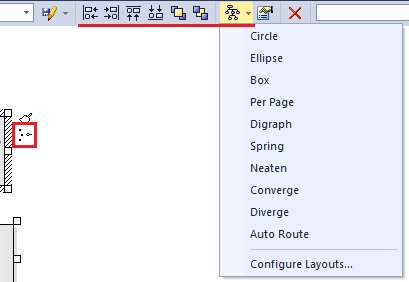
\includegraphics[width=0.65\textwidth]{../../org.moflon.doc.handbook.05_miscellaneous/1_grokkingEA/01_layOutElements/ea_layoutElementsCommonContext}
  \caption{Setting the layout of multiple elements}  
  \label{ea:layout1}
\end{center}
\end{figure}

\begin{figure}[htbp]
\begin{center}  
  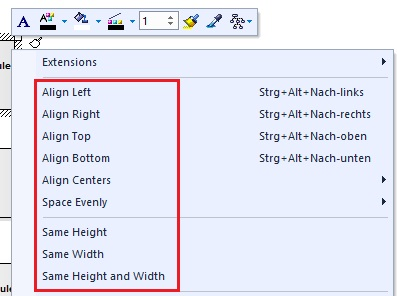
\includegraphics[width=0.7\textwidth]{../../org.moflon.doc.handbook.05_miscellaneous/1_grokkingEA/01_layOutElements/layoutElements2}
  \caption{Further layout options}  
  \label{ea:layout2} 
\end{center}
\end{figure}

\end{stepbystep}


\subsection{Bending lines to your will}

Almost as important as a good layout is getting lines to be just the way you want them to be. In EA you can add and remove bending points which can be used to
control the appearance of a line.

\begin{enumerate}
\item[$\blacktriangleright$]Hold down \texttt{Ctrl} and click on a line to create a bending point (Fig.~\ref{fig_bendLine01}). You can now pull and place the
bending point as you wish.
 
\begin{figure}[htbp]
\begin{center}
  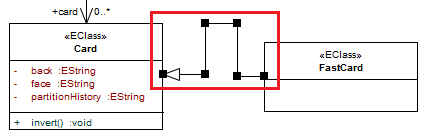
\includegraphics[width=0.8\textwidth]{bendLine1}
  \caption{How to bend lines}   
  \label{fig_bendLine01}
\end{center}
\end{figure}

\item[$\blacktriangleright$] You can create as many bending points as you wish, or \emph{remove} them also by holding down \texttt{Ctrl} and clicking on the
point to be deleted.
\end{enumerate}


\subsection{Deleting vs. removing elements from diagrams} 

A central feature that new users should understand as soon as possible is the way EA handles diagrams. \emph{A diagram is simply treated as a \emph{view} of the
complete model.} The complete model can always be browsed in its entirety via a tree view in the package browser. This space contains all elements that will be
exported. The driving reason behind this setup is that diagrams typically do not contain all elements and one usually uses multiple (possibly redundant)
diagrams to show the different parts of the model. Thinking in this frame is crucial and provides a pragmatic solution to the problem of having huge,
unmaintainable diagrams.

A tricky consequence one must get used to is that removing an element from a diagram does \emph{not} delete it from the model. We have added some support
with the validation in the eMoflon add-in control panel, which can prompt a warning when an element cannot be found in any diagram,\footnote{Review Part II,
Section 2.8 for an example} but there's currently no way to recover a deleted element.

A common mistake new users make is to remove an element by pressing \texttt{del}, and expecting the element to be deleted from the model. As you can probably
guess, this is not the case as evidenced in the package browser (Fig.~\ref{ea:partiallyDeleted}).

\vspace{0.5cm}

\begin{figure}[htbp]
\begin{center} 
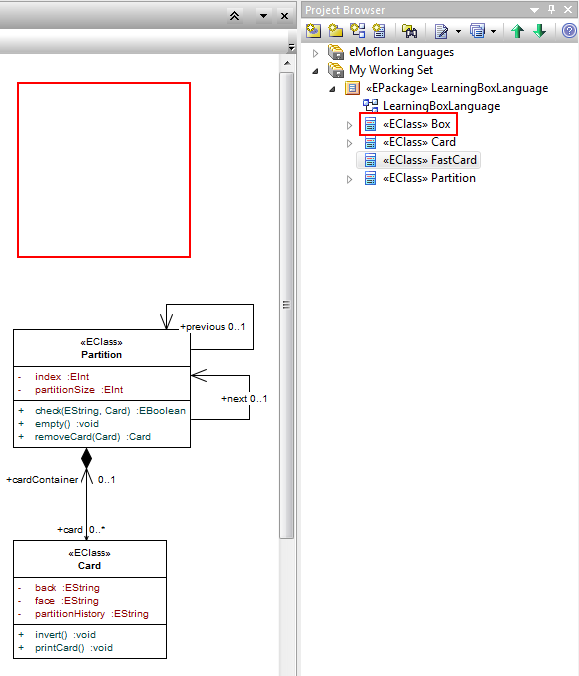
\includegraphics[width=0.6\textwidth]{ea_partiallyDeleted}
  \caption{Removing an element from a diagram via pressing \texttt{Del} does not delete it from the model and it is still present in the package browser}  
    \label{ea:partiallyDeleted}
\end{center}
\end{figure}  

\begin{itemize}
\item[$\blacktriangleright$] To fully delete an element from a model (not just a diagram), select it in the diagram and press \texttt{Ctrl + Del}. Confirm the
action in the warning dialogue (Fig.~\ref{ea:deleteWarning}), and the element should no longer be in the project browser.

\vspace{0.5cm}

\item[$\blacktriangleright$] Alternatively, elements can be deleted directly from project browser by right-clicking the item and navigating to the large
red `x' at the bottom of the context menu

\begin{figure}[htbp]
\begin{center}
  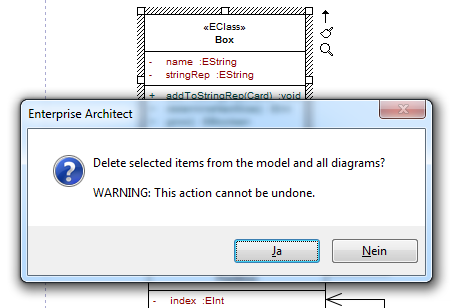
\includegraphics[width=0.7\textwidth]{ea_deleteWarning}
  \caption{Deleting an element from a diagram and the model}  
  \label{ea:deleteWarning}
\end{center}
\end{figure}  

\end{itemize}


\newpage
\subsection{Excluding certain projects from the export}

You may find it sometimes necessary to exclude certain projects from your diagram export (such as the \texttt{MocaTree} model used in Part V).
Some reasons for this could be (i) because the project is still a work in progress and simply not ready to be exported, (ii) because the
complete project is present in the Eclipse workspace but has not been modelled completely in EA, and you wish to do this gradually on-demand, (iii) because the
project is not meant to be present in your Eclipse workspace as generated code and is instead provided via a plugin (this is usually the case for standard
metamodels like Ecore, UML etc.), or (iv) because the project is rather large and stable and you do not want to wait for EA to process a known, unchanging
model. Whatever the reason, you can prevent unnecessary exports by setting a certain \emph{tagged value} of the project.

\begin{enumerate}

\item[$\blacktriangleright$] Open your project in EA, and navigate to ``View/Tagged Values'' from the menu bar (Fig.~\ref{ea:view/Taggedvalues}).

\begin{figure}[htbp]
\begin{center}  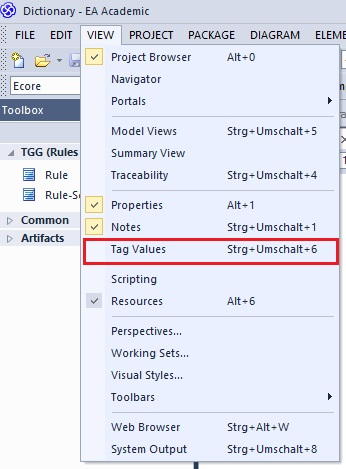
\includegraphics[width=0.5\textwidth]{ea_viewTaggedValues}
  \caption{Opening the tagged values view}  
  \label{ea:view/Taggedvalues}
\end{center}
\end{figure} 

\item[$\blacktriangleright$] The tagged value, \emph{Moflon::Export}, should already be present and be set to a default \texttt{true} value
(Fig.~\ref{ea:moflonExportTG}). If you want the project to be ignored by the eMoflon's validation and/or export functions, change the value to
\texttt{false} (and conversely back to \texttt{true} to export it again).

\begin{figure}[htbp]
\begin{center}
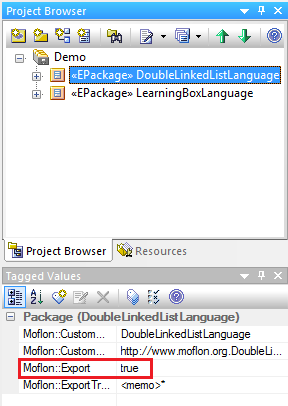
\includegraphics[width=0.5\textwidth]{ea_moflonExportTG}
  \caption{The \texttt{Moflon::Export} setting determines ignored projects}  
  \label{ea:moflonExportTG}
\end{center}
\end{figure}

\end{enumerate}


\subsection{Getting verbose!}

Although we use colours in SDMs to indicate when an element is to be matched (black), created (green), or destroyed (red), it sometimes makes sense to
indicate these binding operators via explicit stereotypes (i.e., for black-and-white printouts of a model).

\begin{enumerate}
  
\item[$\blacktriangleright$] Open the relevant diagram in the EA editor window and, depending on what type it is, press the \texttt{Verbose} button in
either the \texttt{eMoflon SDM Functions} or \texttt{eMoflon TGG Functions} panel (Fig.~\ref{ea:changeVStatus}).

\vspace{0.5cm}

\begin{figure}[htbp]
\begin{center}
  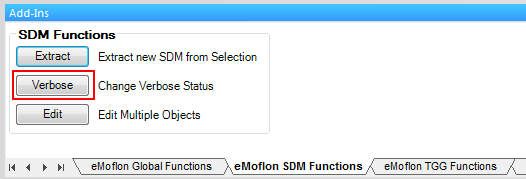
\includegraphics[width=0.8\textwidth]{ea_changeVerboseStatus}
  \caption{Add extra markup to colored links and objects in the current diagram}  
  \label{ea:changeVStatus}
\end{center}
\end{figure}

\item[$\blacktriangleright$] This will add small \texttt{++} or \texttt{-~-} symbols next to deleted and created elements in the current diagram
(Fig.~\ref{ea:verboseSymbols}). Press the button again to deactivate these indicators.

\begin{figure}[htbp]
\begin{center}
  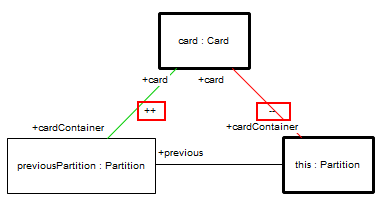
\includegraphics[width=0.7\textwidth]{ea_verboseSymbols}
  \caption{Diagram in verbose mode}  
  \label{ea:verboseSymbols}
\end{center}
\end{figure}

\end{enumerate}


\newpage

\subsection{Duplicating elements via drag-and-drop}

Sometimes you'll have an element (or many) that are nearly identical, and life would be \emph{so} much easier if you could copy and paste an existing one
already. Suppose you want a copy of a \emph{this} element, so you press \texttt{ctrl + C}, followed by \texttt{ctrl + v}. An error dialogue preventing the
action will immediately raise, stating that the ``\ldots diagram already contains an instance of the element you are trying to paste.'' EA can only support
unique objects, so you'll need to use the following process.

\begin{itemize}

\item[$\blacktriangleright$] In either a diagram or in the project browser, hold \texttt{ctrl}, then drag the element you wish to duplicate. A
confirmation-style dialogue will appear (Fig.~\ref{ea:dupWindow}), and a properties window will follow. You must assign a unique name to the new element, or
else you'll receive an error when you try to export the project later.

\begin{figure}[htbp]
\begin{center}
  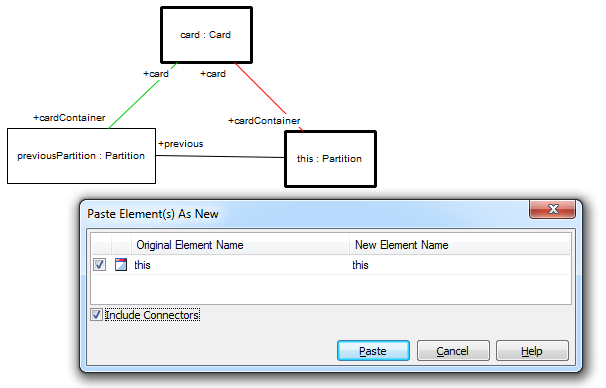
\includegraphics[width=0.95\textwidth]{ea_duplicatingElements}
  \caption{Copying new elements}  
  \label{ea:dupWindow}
\end{center}
\end{figure}

\end{itemize}


\newpage

\hypertarget{subsec:seekAndFind}{}

\subsection{Seek, and ye shall find \ldots}

EA has a model search function that can be quite handy for large models with thousands of elements and a brain that just can't remember where something is. 

\begin{enumerate}

\item[$\blacktriangleright$]Select ``Model Search Window'' and enter the name of an element you wish to find (Fig.~\ref{fig_search01}).\footnote{You can also
access this window by pressing \texttt{ctrl+alt+A}} 

\begin{figure}[htbp]
\begin{center}
  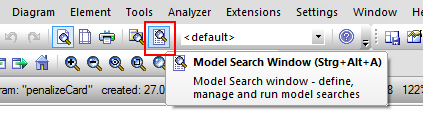
\includegraphics[width=0.63\textwidth]{search1}
  \caption{Model Search Window}  
  \label{fig_search01}
\end{center}
\end{figure}

\item[$\blacktriangleright$] All elements that meet the search criteria are listed and you can right-click on each of the items and select one of the options
above to locate the element.

\item[$\blacktriangleright$] In a similar way, you can locate the corresponding class of an object by right clicking and selecting ``Find/Locate Classifier in
Project Browser.''

\end{enumerate}


\subsection{Advanced search}
\label{sect:appendix_adv_search}

EA offers an even more advanced search capability using SQL\footnote{For some detailed insights to the general database schema used by EA cf. \\
\url{http://www.sparxsystems.com.au/downloads/corp/scripts/SQLServer_EASchema.sql}}.
To make use of this option, go to the model search dialog (\mbox{Ctrl+Alt+A}). Click on the ``Builder'' button and switch to the SQL-tab. Here you can 
formulate any query on the underlying database. The SQL-editor helps you with syntax-highlighting and auto-completion. Here are some basic examples:

\begin{enumerate}
\item[$\blacktriangleright$]
To find all eClasses
\begin{lstlisting}[frame=single,framerule=0pt]
SELECT * FROM t_object
WHERE Object_Type='Class' AND Stereotype='eclass';
\end{lstlisting}

\item[$\blacktriangleright$]
To find all associations
\begin{lstlisting}[frame=single,framerule=0pt]
SELECT * FROM t_connector
WHERE Connector_Type='Association';
\end{lstlisting}

\item[$\blacktriangleright$]
To find all inheritance relations
\begin{lstlisting}[frame=single,framerule=0pt]
SELECT * FROM t_connector
WHERE Connector_Type='Generalization';
\end{lstlisting}

\item[$\blacktriangleright$]
To find all connectors attaching a note to an element
\begin{lstlisting}[frame=single,framerule=0pt]
SELECT * FROM t_connector
WHERE Connector_Type='NoteLink';
\end{lstlisting}

\item[$\blacktriangleright$]
To find all control flow edges (used in SDMs)
\begin{lstlisting}[frame=single,framerule=0pt]
SELECT * FROM t_connector
WHERE Connector_Type='ControlFlow';
\end{lstlisting}

\item[$\blacktriangleright$]
To find all associations connected to a class named ``EClass''
\begin{lstlisting}[frame=single,framerule=0pt]
SELECT t_object.Name, t_connector.* FROM t_connector,t_object
WHERE t_connector.Connector_Type='Association'
  AND (t_connector.Start_Object_ID=t_object.Object_ID
    OR t_connector.End_Object_ID=t_object.Object_ID)
  AND t_object.Name='EClass';
\end{lstlisting}

\item[$\blacktriangleright$]
To determine all subtypes of ``EClassifier''
\begin{lstlisting}[frame=single,framerule=0pt]
SELECT a.Name FROM t_connector,t_object a,t_object b
WHERE t_connector.Connector_Type='Generalization'
  AND t_connector.Start_Object_ID=a.Object_ID
  AND t_connector.End_Object_ID=b.Object_ID
  AND b.Name = 'EClassifier';
\end{lstlisting}

\item[$\blacktriangleright$]
To determine all supertypes of ``EClassifier'' (cf. above)
\begin{lstlisting}[frame=single,framerule=0pt]
...
  AND t_connector.Start_Object_ID=b.Object_ID
  AND t_connector.End_Object_ID=a.Object_ID
...
\end{lstlisting}
\end{enumerate}

To run the search, either hit the run button in the upper left corner of the editor (it shows a triangular shaped ``play'' pictogram) or punch \texttt{F5} on
your keyboard.

\clearpage


\newpage
\section{Using Enterprise Architect with Subversion}
\visHeader

The following steps are required to setup EA for use with subversion. This is highly recommended when working in a group and sharing a single EA Project (EAP)
file, which is otherwise a huge binary blob. We assume you wish to use (i) Subversion and (ii) Windows. For other SCM and operating systems please consult the
official documentation from EA.



\subsection{Initial preparation and set-up}

Download and install Slik SVN (mandatory):
\begin{enumerate}
  \item[$\blacktriangleright$] x32: \small{\url{http://www.sliksvn.com/pub/Slik-Subversion-1.7.6-win32.msi}}\\\\
   x64: {\small \url{http://www.sliksvn.com/pub/Slik-Subversion-1.7.6-x64.msi}}
\end{enumerate}

For public/private key authentication, you also need Tortoise SVN:

\begin{enumerate}
  \item[$\blacktriangleright$] x32: {\small \begin{minipage}{.95\textwidth} 
  \url{http://sourceforge.net/projects/tortoisesvn/files/1.7.9/Application/TortoiseSVN-1.7.9.23248-win32-svn-1.7.6.msi/download}
    \end{minipage}}\\\\\\
  x64: {\small\begin{minipage}{.9\textwidth} 
  \url{http://downloads.sourceforge.net/project/tortoisesvn/1.7.9/Application/TortoiseSVN-1.7.9.23248-x64-svn-1.7.6.msi/download}\end{minipage}}
\end{enumerate}

If you do not want to have your private key password in plain text in an SVN configuration file then also download Pageant:
\begin{enumerate}
  \item[$\blacktriangleright$] {\small \url{http://the.earth.li/~sgtatham/putty/latest/x86/pageant.exe}}
\end{enumerate}

After installing all the tools we need, we now have to setup the SSH tunnel:

\begin{enumerate}
  \item[$\blacktriangleright$] Locate the file \texttt{\%APPDATA\%$\backslash$Subversion$\backslash$config} and open it with your favourite editor. Locate the
  \texttt{[tunnels]} section.
  \item[$\blacktriangleright$] If you do not want to install Pageant and do not mind entering your password in plain text enter the following command:\\
  \texttt{ssh = "<path to Tortoise SVN>/bin/TortoisePlink.exe" -l \\<username> -pw <password for your private key> -i "<path to your private key>"}
  \item[$\blacktriangleright$] If you wish to use Pageant then the command can be simplified to:\\ \texttt{ssh = "<path to Tortoise SVN>/bin/TortoisePlink.exe"
  -l \\<username>} as you can add your private key to Pageant.
  \item[$\blacktriangleright$] If you just use direct passwords for authentication then you can leave out the \texttt{-i} option in both cases.
\end{enumerate}



\subsection{How to set-up a version controlled EAP file}

In the following we assume an EAP file has already been placed under version control \emph{according to our tutorial} and that you wish to check-out this file
and work with it. If our instructions do not work, the EAP file might have been placed under version control in a different manner. If this is the case then
please contact whoever checked-in the file and set it up for working with EA and SVN for further instructions.

\begin{enumerate}
  \item[$\blacktriangleright$] Check-out the project with the EAP file from the server using Tortoise-SVN or Eclipse/Subclipse (or any SVN client of your
  choice). You should now have a \textit{.svn}-folder in the directory where you saved the revision.
  \item[$\blacktriangleright$] Open the EAP file. If the EAP file is already under version control \emph{and has been set-up correctly}, a dialogue similar to
  Fig.~\ref{fig:advanced-topics-eaSVN-incompleteConf} should immediately pop-up.
  \item[$\blacktriangleright$] Click ``Yes" to open the ``Version Control Settings'' dialogue (Fig.~\ref{fig:advanced-topics-eaSVN-setWorkingCopyPath}).

\begin{figure}[!htbp]
\begin{center}
	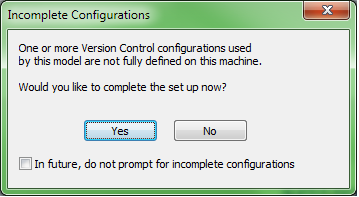
\includegraphics[width=0.5\textwidth]{011}
	\caption{Configure an EAP file which is already under version control}
  	\label{fig:advanced-topics-eaSVN-incompleteConf}
\end{center}
\end{figure}

   \item[$\blacktriangleright$] To work with the EAP file, you now have to \emph{redefine} the SVN variable for the file in your EA workspace.
   To accomplish this, choose the local path to the folder which contains the EAP file in the ``Working Copy Path'' text-box, and correct the value in
   ``Subversion Exe Path'' if necessary (to fit your Slik installation location).

\begin{figure}[!htbp]
\begin{center}
	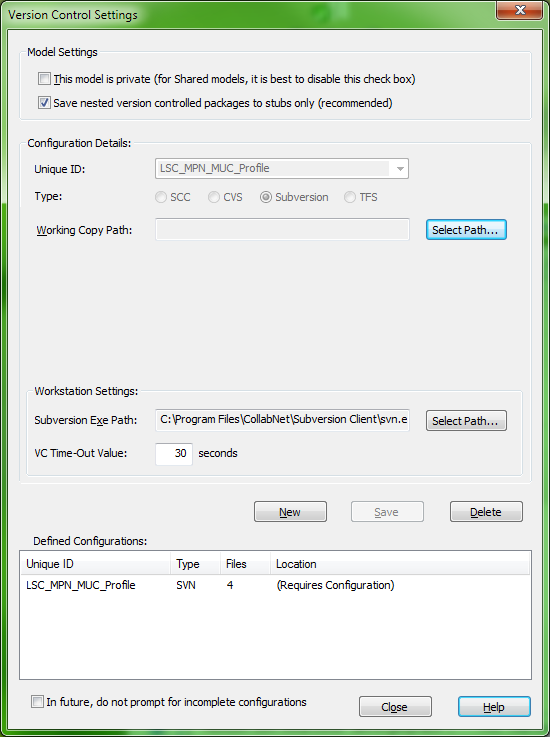
\includegraphics[width=0.5\textwidth]{012}
	\caption{Update settings as required}
  	\label{fig:advanced-topics-eaSVN-setWorkingCopyPath}
\end{center}
\end{figure}

\end{enumerate}



\subsection{Working with a version controlled EAP file}
\label{sect:appendixB_update_commit}

\begin{enumerate}
  \item[$\blacktriangleright$] A \texttt{Check Out} retrieves the lock for a certain package and gives you exclusive access, i.e., no one else can change the
  package. Very important: if subpackages are also under version control, they are not affected by checking out the ``super''-package and remain locked.
  A \texttt{Check Out} also updates the package to the latest version.

\item[$\blacktriangleright$] A \texttt{Check In} commits your work to the server and gives up the lock on the package so others can work on it.
If you do not want to commit your changes, you can just use \texttt{Undo Check Out...} to revert all local changes.

\item[$\blacktriangleright$]  The corresponding \texttt{..Branch} options perform the actions for the current package and all subpackages.
Please note, this has nothing to do with ``branching'' in normal SVN lingo.

\item[$\blacktriangleright$] \texttt{Get Latest/Get All Latest} retrieves the latest version of the selected package / all packages.
This is basically an update but does not retrieve the lock for any package.

\item[$\blacktriangleright$] Conversely, \texttt{Put Latest} saves all your changes without giving up any locks.

\item[$\blacktriangleright$] \texttt{Compare with controlled version} can be used to review incoming changes.
Green elements will be added, red will be deleted.

\item[$\blacktriangleright$] \texttt{File History} gives you a summary of all commits made while you were lying on the beach.
For a useful file history, always use meaningful commit statements when checking in!
A date stamp is created automatically.
\end{enumerate}



\subsection{Placing an EAP file under version control}
\label{sect:appendixB_new_EAP_for_vc}

If you already have an EAP file and would like to place it under version control, you first have to check it in as usual on the server using your favourite SVN
client. Once the project is checked in, the required .svn folder should be in the folder containing the EAP file. The next step is to register an SVN-variable
in EA:

\begin{enumerate}
  \item[$\blacktriangleright$] Open the EAP file, right click on a root folder and select ``Package Control'' and then ``Version Control Settings...''
  (Fig.~\ref{fig:advanced-topics-eaSVN-rightclick}).
  
\begin{figure}[!htbp]
\begin{center}
 	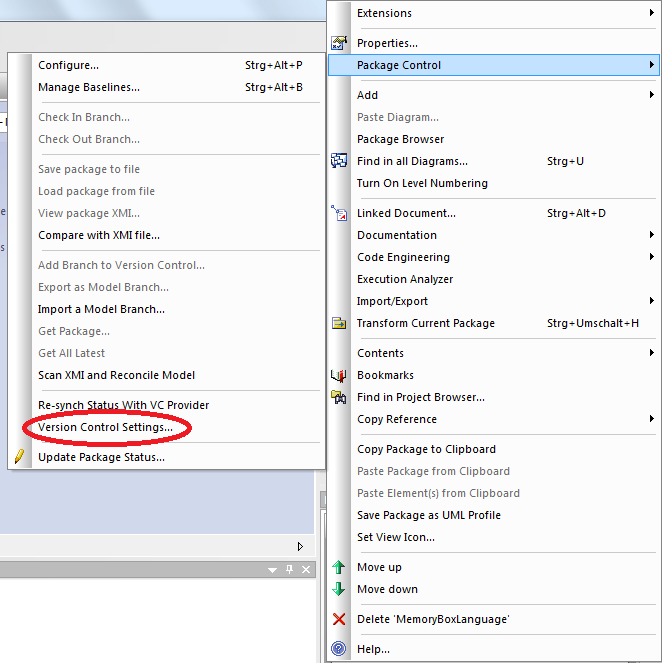
\includegraphics[width=0.7\textwidth]{rightclick}
	\caption{Select version control settings}
  	\label{fig:advanced-topics-eaSVN-rightclick}
\end{center}
\end{figure}

  \item[$\blacktriangleright$] In the dialogue, choose a unique ID of your choice (we suggest you use the name of the EAP file) for the settings and activate
  the ``Subversion'' radio button below.
  \item[$\blacktriangleright$] Choose the local path to the folder which contains the EAP file in the ``Working Copy Path'' text-box.
  \item[$\blacktriangleright$] The field ``Working Station'' must point to where you installed Sliksvn, i.e., \texttt{<path to
  SlikSVN>$\backslash$bin$\backslash$svn.exe")}. Press ``Save'' and close the dialogue (Fig.~\ref{fig:advanced-topics-eaSVN-variable}). If the dialogue closes
  without an error message, then you can be sure to have configured everything correctly.

%\usepackage{graphics} is needed for \includegraphics
\begin{figure}[!htbp]
\begin{center}
	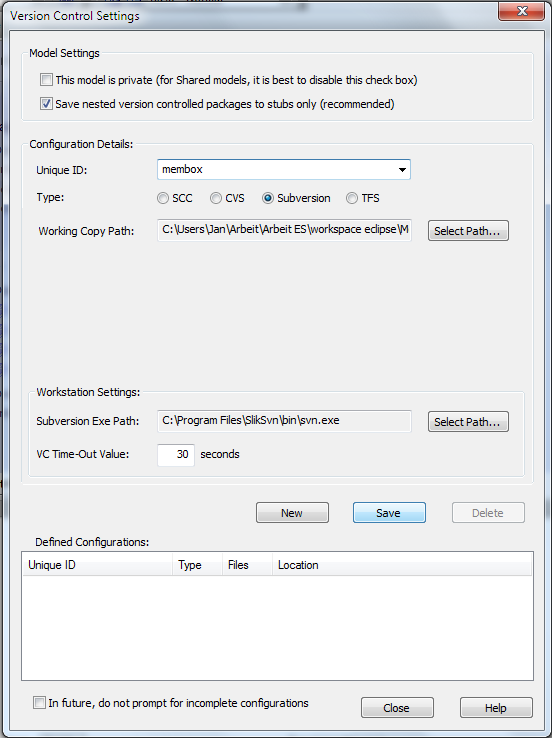
\includegraphics[width=0.6\textwidth]{versioncontrol}
	\caption{Register an SVN variable in EA}
  	\label{fig:advanced-topics-eaSVN-variable}
\end{center}
\end{figure}

\item[$\blacktriangleright$] In the EAP file, choose ``Package Control$\backslash$Configure...'' for \emph{each package} you wish to place under version control.

\item[$\blacktriangleright$] In the ensuing dialogue, activate ``Control Package'' and select your previously defined SVN variable from the drop-down menu.
Enter the path where the XML file for the project should be placed. Although this is not enforced in any way, we recommend you create a folder structure that
mirrors the package structure in EA (Fig.~\ref{fig:advanced-topics-eaSVN-addPackage}). This process has to be repeated \emph{for all sub-packages} as soon as
their super-package has been placed under version control.

\begin{figure}[!htbp]
\begin{center}
	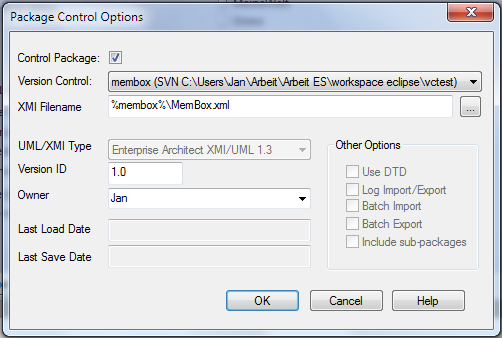
\includegraphics[width=0.6\textwidth]{cont}
	\caption{Placing a package under version control}
  	\label{fig:advanced-topics-eaSVN-addPackage}
\end{center}
\end{figure}

\item[$\blacktriangleright$] As a final step, check-in the current state of the EAP file directly with your SVN client.
As from this point, the EAP file should not be checked-in anymore, and all versioning actions should be performed via EA (and not directly with your SVN
client).
\end{enumerate}
\clearpage

\newpage

\section{Using Existing EMF Projects in eMoflon}
\visHeader

This chapter contains stepwise instructions on how to use existing \mbox{EMF}/\-Ecore projects with an eMoflon project.  As an example, we shall implement a
small subset of the \texttt{Ecore -> GenModel} transformation. The \emph{GenModel} for a given Ecore model can be viewed as a \emph{wrapper} that contains
additional Java code generation specific details. These details are separated from the Ecore model to keep it free of such ``low-level'' information and
settings.

As the metamodel for \texttt{GenModels} is part of the EMF/Ecore standard, this is an example of an existing metamodel which must be integrated in eMoflon
before you can, for example, specify the transformation using SDMs.
Based on this example, the basic workflow for using an existing EMF project in eMoflon is described in the following.

\section{Modelling relevant aspects in EA}
\genHeader

The first step is to load an existing metamodel into EA. A complete and automatic import of existing Ecore files in EA is currently not possible and therefore,
\emph{relevant parts} of the existing metamodel (\texttt{GenModel}) have to be modelled manually. Although this might sound frightening (especially for
large, complex metamodels), the emphasis here on \emph{relevant} indicates that only elements that are needed for the transformation have to be present in
EA, where more can be added iteratively as the transformation grows. 

If you find this section challenging or unclear, refer to Part II: Ecore for a detailed review of metamodel construction.

\begin{stepbystep}

\item Open Eclipse and create a new metamodel project named \texttt{Ecore\-To\-Gen\-Model}, do not select the \texttt{Add Demo Specification}
option in the project wizard window.

\item A new specifications folder with the project name should have been loaded into the workspace.

\item Double-click the generated \texttt{Ecore\-To\-Gen\-Model.eap} file to open your project in EA. 
Explore the project browser and make note of the packages already present in EA under \texttt{eMoflon Languages}, especially \texttt{Ecore} which we shall use in this transformation.

\item Select the root note \texttt{My Working Set} and create a new package named \texttt{Gen\-Model\-Language}. 

\item Add a new Ecore diagram and model the elements as depicted in \Cref{fig_gMM}. You'll need to create the three EClasses on
the left, but \texttt{Ecore::EPackage} and \texttt{Ecore::EClass} are to be drag-and-dropped and pasted as links from the project browser. 

\vspace{0.5cm}

\begin{figure}[htbp]
\begin{center}  
	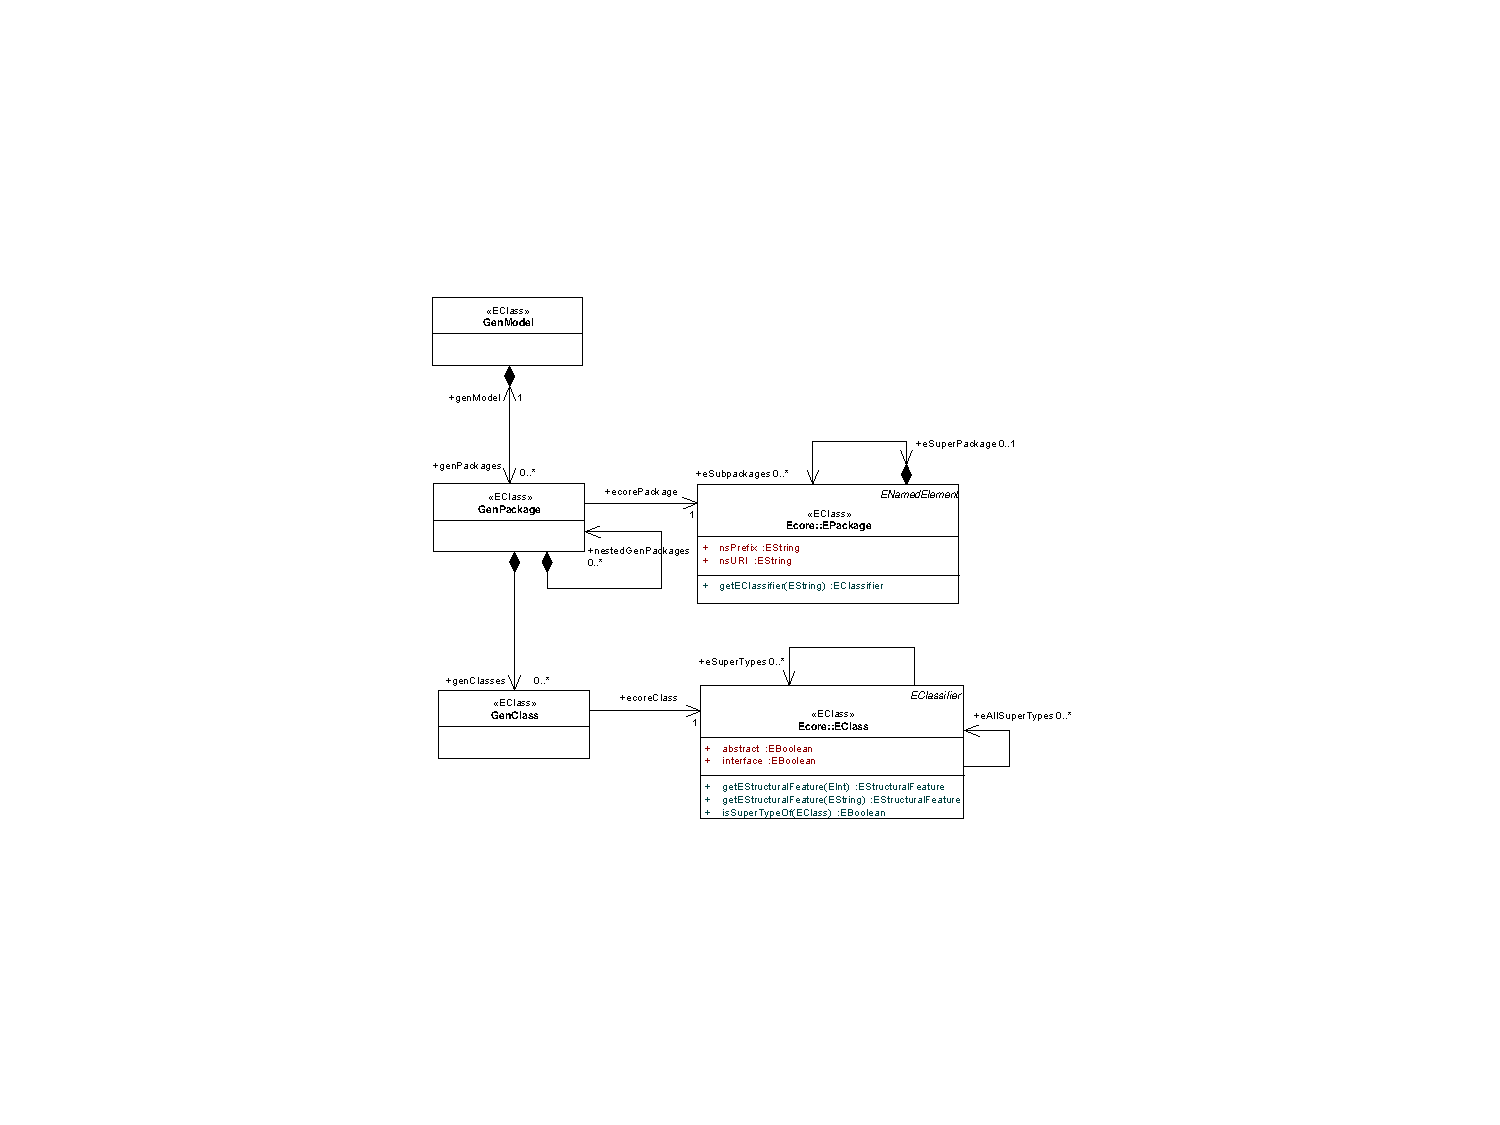
\includegraphics[width=\textwidth]{../../org.moflon.doc.handbook.05_miscellaneous/3_existingEMF/emfImages/CDGenmodel.pdf}
	\caption{Metamodel of \texttt{GenModel}}  
\label{fig_gMM}
\end{center}
\end{figure} 

\vspace{0.5cm}

\item Please note that the actual \texttt{GenModel} metamodel contains many more elements, but this subset is sufficient for our
task.
Although this subset can be incomplete, it must be correct and not contradict the actual \texttt{GenModel} metamodel in any way!

\item Navigate to the project browser again and create another package named \texttt{Ecore2GenModel}.  
This will contain the \texttt{Transformer} class; Create and complete its Ecore diagram as depicted in \Cref{fig_e2gm}.

\item Carefully double-click each method to create and implement their SDMs as depicted in \Cref{fig_pack2g,fig_transf}.
\end{stepbystep}

\newpage

\vspace*{2cm}

\begin{figure}[htbp]
	\begin{center}  
	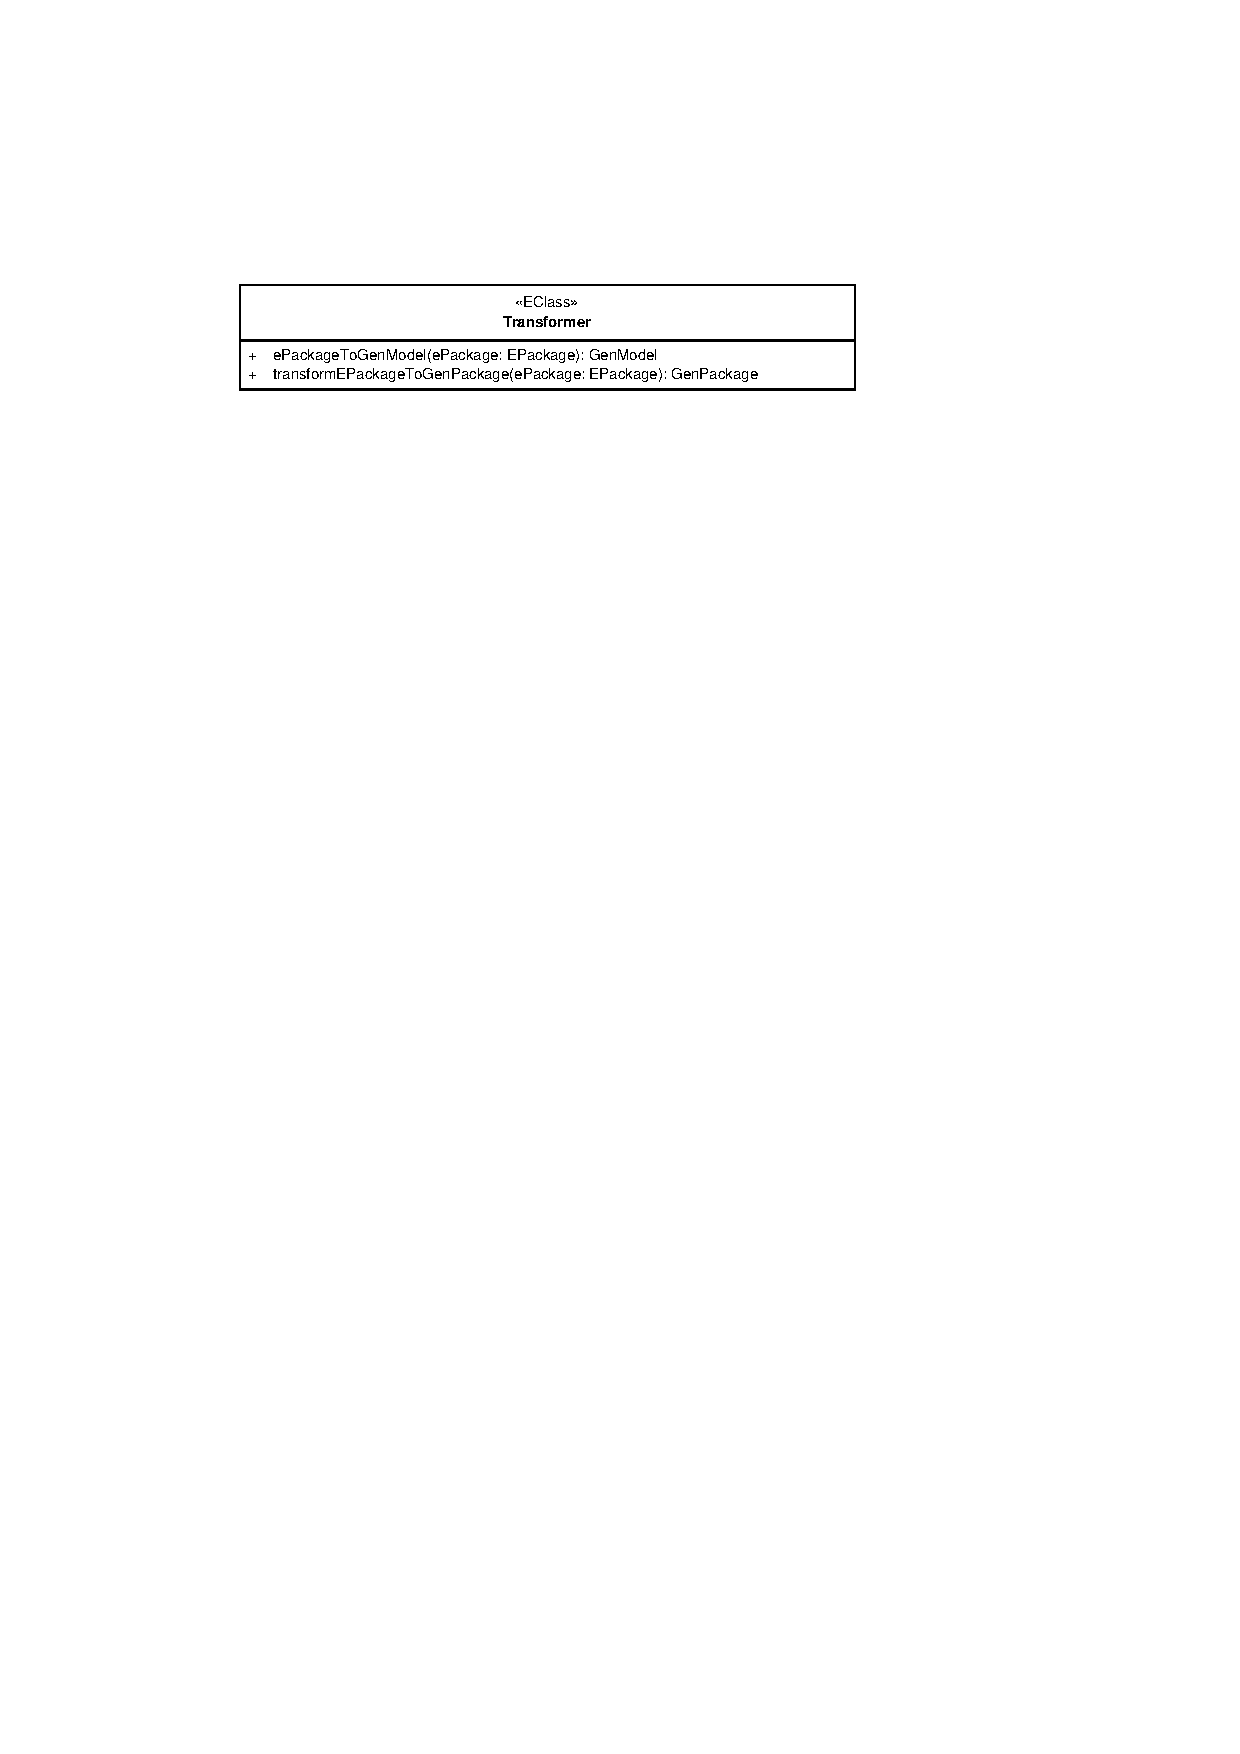
\includegraphics[width=0.7\textwidth]{../../org.moflon.doc.handbook.05_miscellaneous/3_existingEMF/emfImages/CDTransformer.pdf}
	\caption{Methods in \texttt{Transformer}}  
	\label{fig_e2gm}
	\end{center}
\end{figure} 

\vspace{1cm}

\begin{figure}[htbp]
\begin{center}  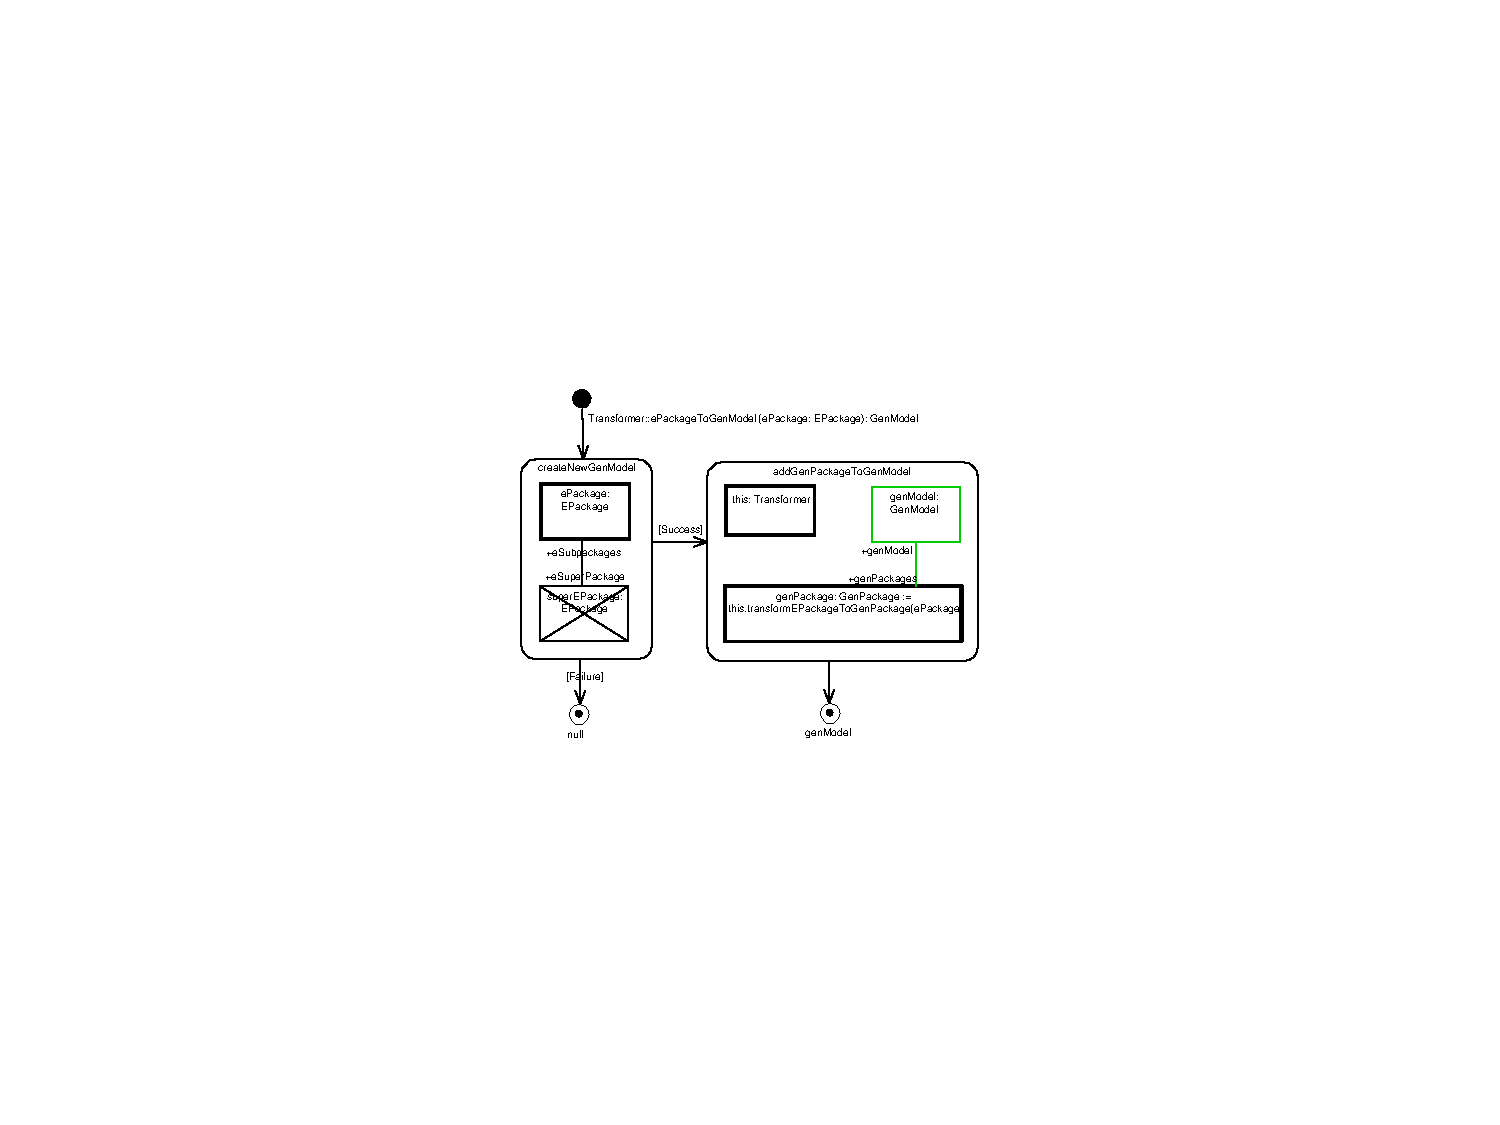
\includegraphics[width=0.8\textwidth]{../../org.moflon.doc.handbook.05_miscellaneous/3_existingEMF/emfImages/SDMePackageToGenModel.pdf}
        \caption{Main method for \texttt{EPackage} to \texttt{GenModel} transformation}  
  \label{fig_pack2g}
\end{center}
\end{figure} 

\begin{figure}[htbp]
\begin{center}  
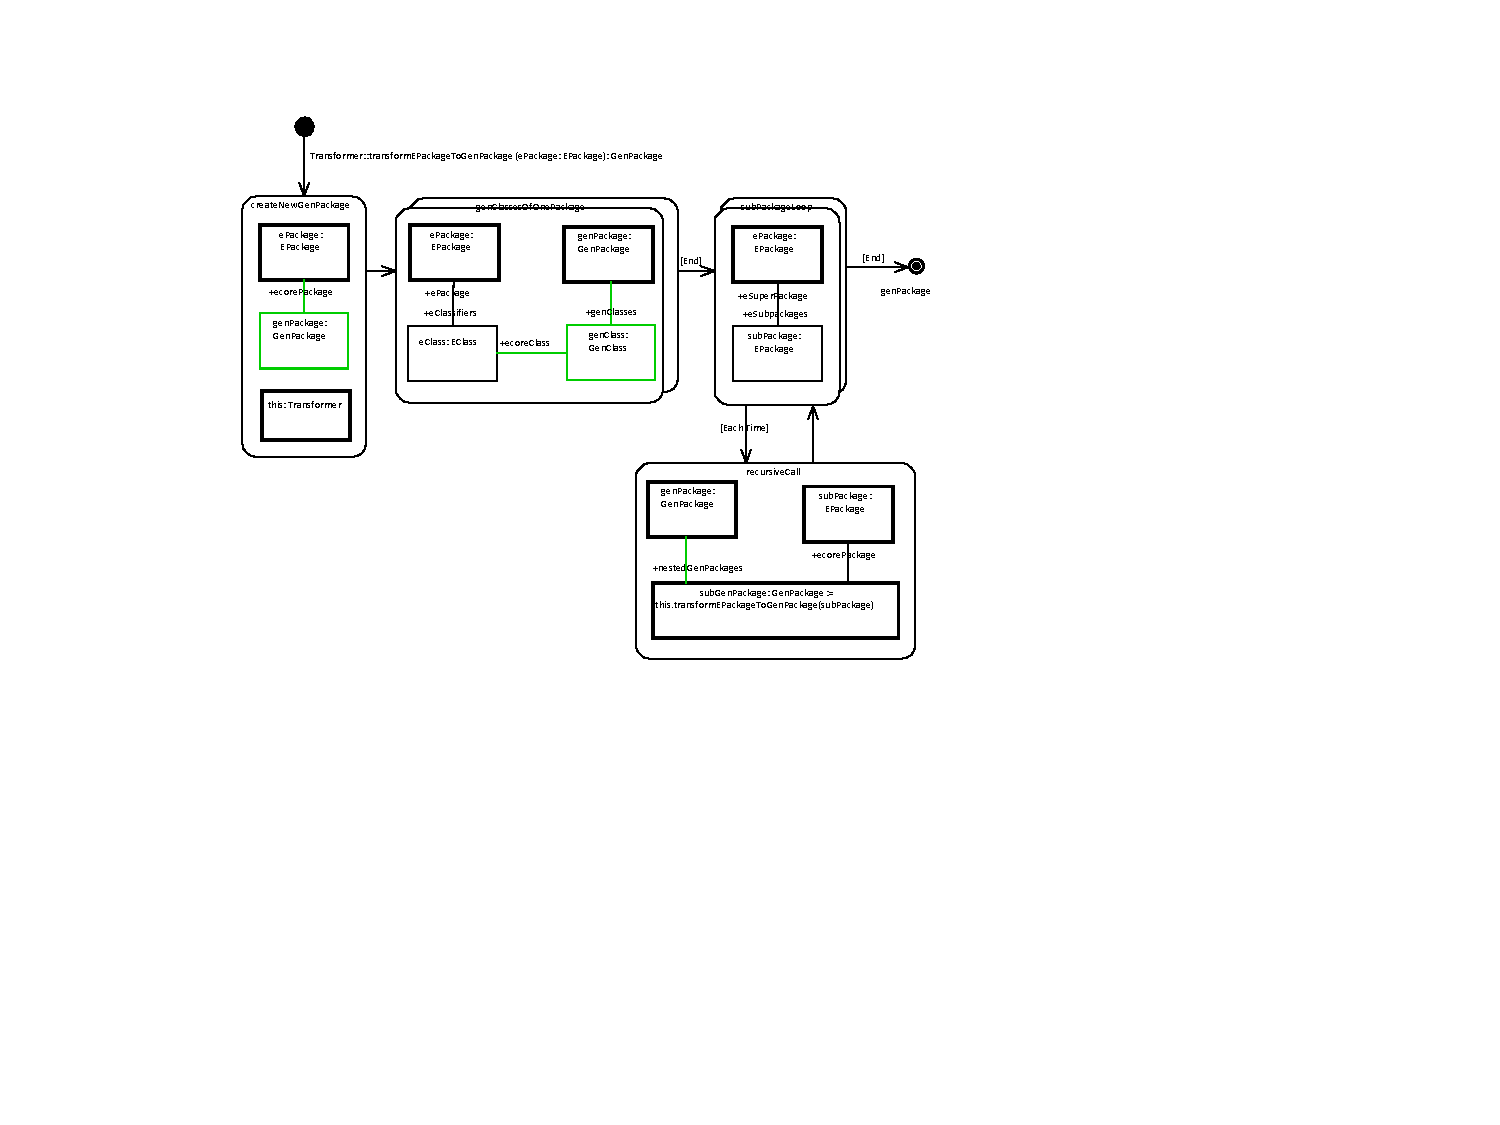
\includegraphics[width=1.1\textwidth]{../../org.moflon.doc.handbook.05_miscellaneous/3_existingEMF/emfImages/SDMtransformEpackageToGenPackage.pdf}
\caption{Helper function to transform all \texttt{EPackages} to \texttt{GenPackages}}  
\label{fig_transf}
\end{center}
\end{figure} 



\newpage

\subsection{Configuration for code generation in Eclipse}
\genHeader

Since there is already generated code for the existing \texttt{GenModel} metamodel (provided via the Eclipse plugin), we do \emph{not} want to export our
incomplete subset of \texttt{GenModel} from EA. Instead, we need to configure Eclipse to access the elements specified in our partial metamodel from the
complete metamodel.

\begin{enumerate}

\item[$\blacktriangleright$] In EA, right-click your \texttt{GenModelLanguage} package and select ``Properties\ldots'' 

\item[$\blacktriangleright$] Navigate to ``Properties/Moflon'' in the dialogue window and update the tagged \texttt{Moflon::Export} value to \texttt{false}
(Fig.~\ref{fig_customNS}).

\vspace{0.5cm}

\begin{figure}[htb]
\begin{center}  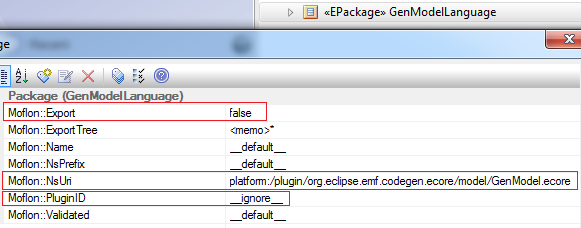
\includegraphics[width=\textwidth]{ea_genModelExportFalse}
  \caption{Update the \texttt{GenModel} export option and create custom tags}  
  \label{fig_customNS}
\end{center}
\end{figure}

\newpage

\item[$\blacktriangleright$] Next we have to set the ``real'' name and URI of the project to be used in Eclipse so that the relevant references are exported
properly. In the same window, create new tagged values \texttt{Moflon::CustomNsPrefix} and \texttt{Moflon::CustomNsUri}.

\item[$\blacktriangleright$] Set their values to \texttt{genmodel} and \texttt{http://\-www.\-eclipse.\-org/\-emf/\-2002/\-GenModel} respectively, as shown in
Fig.~\ref{fig_customNS}. These values can be determined by inspecting the corresponding values in the existing .ecore file (i.e.,~the existing metamodel).

\item[$\blacktriangleright$] Validate and export all projects as usual to your Eclipse workspace, and update the metamodel project by pressing \texttt{F5} in
the package explorer.

\item[$\blacktriangleright$] In order to simplify setting the required dependencies for code generation,  convert the generated Eclipse project
\texttt{Ecore2GenModel} to a \emph{plug-in project} by right-clicking the project and selecting ``Configure/Convert to Plug-in Projects...''

\item[$\blacktriangleright$] Right-click \texttt{Ecore2GenModel} once more and navigate to ``Plug-in Tools/Open Manifest.'' The plug-in manager should have
opened in the editor with a series of tabs at the bottom for each option.

\item[$\blacktriangleright$] Switch to the \texttt{Dependencies} tab. Press \texttt{Add} and enter \texttt{org.\-eclipse.\-emf.\-codegen.\-ecore}. This plug-in
includes both the \texttt{Ecore} and \texttt{Gen\-Mod\-el} libraries we require.

\end{enumerate}

Although we have already specified the name and URI of the existing project (in this example, \texttt{GenModel}) as tagged project values, we now have to tell
eMoflon where to find the correct implementation (generated code) of the existing project.

\begin{enumerate}
  
\item[$\blacktriangleright$] Expand the \texttt{Ecore2GenModel} project folder and open the \texttt{mof\-lon.\-prop\-er\-ties.\-xmi} file tree. Right-click the
properties container, and create a new \texttt{Add\-it\-ion\-al Dep\-en\-den\-cies} child. Double click the element to open its properties tab below the
editor, and as shown in Fig.~\ref{eclipse:addDepChild}, update its \texttt{Value} to:\\
\end{enumerate}

\vspace{-1cm}
{\small \ttfamily  platform:/plugin/org.eclipse.emf.codegen.ecore/model/GenModel.ecore} \\
\vspace{-0.5cm}

\begin{figure}[htbp]
\begin{centering}
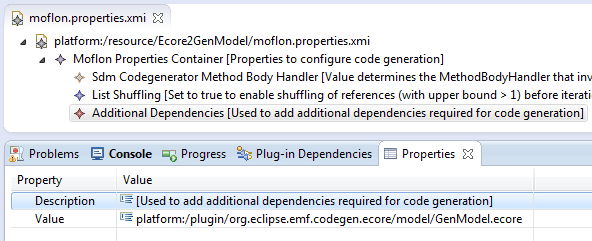
\includegraphics[width=\textwidth]{eclipse_additDepProps}
  \caption{Setting properties for the correct implementation code}  
  \label{eclipse:addDepChild}
\end{centering}
\end{figure} 

\begin{enumerate}

\item[$\blacktriangleright$] Similarly, add a second \texttt{Additional Used Gen Packages} child and set its value to: \\
\end{enumerate}

\vspace{-1cm}
{\small \ttfamily platform:\-/\-plugin/\-org.\-eclipse.\-emf.\-codegen.\-ecore/\-model/\-GenModel.\-genmodel}

\newpage
Finally, to compenstate for some cases where our naming conventions were violated, analogously add the following mapping as corrections:

\begin{enumerate}
\item[$\blacktriangleright$] Add an \emph{import mapping} child for correct generation of the required import, setting the key as \texttt{genmodel} (as
depicted in Fig.~\ref{eclipse:impMapValues}) and value to: \\
{\small \ttfamily \hspace*{1.5cm} org.\-eclipse.\-emf.\-codegen.\-ecore.\-genmodel}

\vspace{0.5cm}

\begin{figure}[htbp]
\begin{centering}
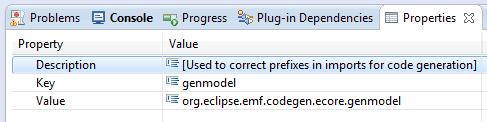
\includegraphics[width=0.9\textwidth]{eclipse_importMappingValues}
  \caption{Mapping properties from our metamodel to the existing \texttt{GenModel}}  
  \label{eclipse:impMapValues}
\end{centering}
\end{figure} 

\item [$\blacktriangleright$] Finally, add a \emph{factory mapping} to ensure that \texttt{GenModelFactory} is used as the factory for creating elements in the
transformation instead of \texttt{Genmodel\-Factory}, which would be the default convention. Set its key as \texttt{genmodel}, and its value to:
{\small \ttfamily GenModelFactory}.

\item [$\blacktriangleright$] Your completed \texttt{moflon.properties.xmi} file should now closely resemble Fig.~\ref{eclipse:finalPropTree}. Refresh your
workspace one more time to generate code for the project and ensure that the transformation behaves as expected via a JUnit test.

\newpage

\vspace*{2cm}

\begin{figure}[htbp]
\begin{centering}
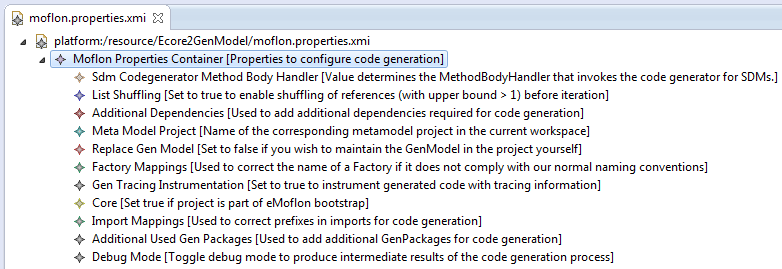
\includegraphics[width=\textwidth]{eclipse_finalPropTree}
  \caption{Additional properties for code generation}  
  \label{eclipse:finalPropTree}
\end{centering}
\end{figure} 

\end{enumerate}



\newpage

\section{The transformation protocol}

\genHeader

If you worked through Part IV of the handbook, you'll remember that we introduced \emph{bidirectional model transformations} via Triple Graph Grammars
(TGGs). These take an instance input model and apply a series of rules to generate a transformed output model and correspondence (or link) metamodel.
Together, these three files form the transformation's \emph{graph triple}. You might also remember that we introduced an integrator in
Section 6, a visualizing tool that can help you trace a transformation via the correspondence model. 

While the integrator's display structure is based on the entire graph triple, its purpose is to interpret the key parts of the transformation's co-generated
\texttt{protocol} file, the detailed listing of every executed action. As you can imagine, examining this file directly provides much more detail than the
integrator alone. While both list the current step, element, rule candidates, and their results, the protocol includes properties of each step such as the
current element's full name, a listing of the created and/or translated elements, the reasons for a rule's success for failure, and other information.

To help us explain, let's revisit the running example as it was in Part IV, Section 7, where a fourth partition and card were added to a forward
transformation only able to handle three partitions. Let's start by reviewing the integrator as shown in Fig.~\ref{eclipse:integratorFWD}.

\begin{figure}[htbp]
\begin{center} 
  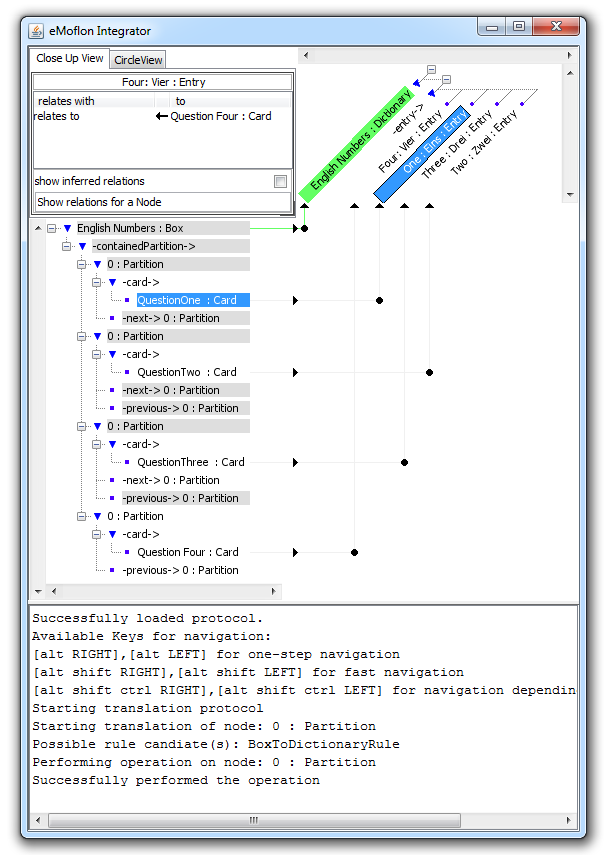
\includegraphics[width=0.8\textwidth]{eclipse_successBoxToDictionaryIntegrator}
  \caption{Integrator view of successful \texttt{BoxToDictionaryRule}}  
  \label{eclipse:integratorFWD}
\end{center}
\end{figure}

It begins the process by trying to translate the first node in the box, \texttt{part\-it\-ion\-0}. It checks for and applies the only valid rule, where each
navigation step shows the operation being executed in the display window. The final message tells us the rule was successful! Remember,
\texttt{BoxToDictionaryRule}\footnote{Refer to Part IV, Section 4, Fig. 28 (Visual) and Fig. 37 (Textual)} creates the primary container elements, \texttt{Box}
and \texttt{Dictionary}, and translates up to three connected \texttt{partitions}.

\newpage

Now let's see the equivalent transformation in the protocol file as depicted in Fig.~\ref{eclipse:protocolFWD}.

\vspace{0.5cm}

\begin{figure}[htbp]
\begin{center} 
  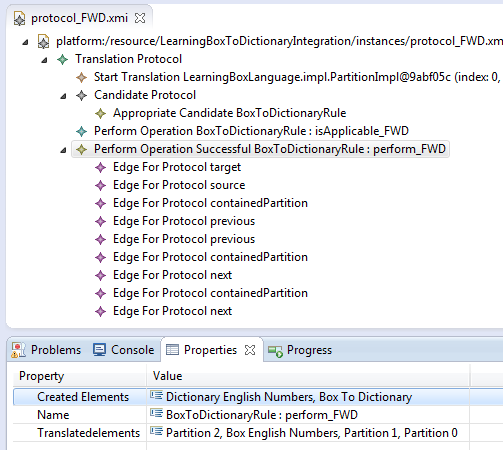
\includegraphics[width=0.9\textwidth]{eclipse_successBoxToDictionaryProtocol}
  \caption{Protocol file of successful \texttt{BoxToDictionaryRule}}  
  \label{eclipse:protocolFWD}
\end{center}
\end{figure}

Again, the translation starts with the zero node (identified by its \texttt{index}) and finds a valid rule. It performs the rule, and lists its final result.
More information can be found however by double-clicking the success node, where the \texttt{Properties} window lists every element that was created and
translated. Finally expanding this successful node, we can then see further details about every edge that needed to be handled which in turn include details
such as their \texttt{name}, \texttt{Source}, and \texttt{Target} elements.

Let's skip ahead to something more interesting. Let's examine the place where the transformation starts trying to handle the erroneous fourth partition
(Fig.~\ref{eclipse:fourthPartition}).

\newpage

\begin{figure}[htbp]
\begin{center} 
  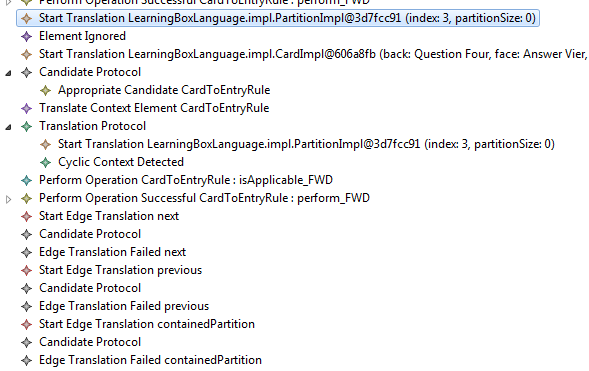
\includegraphics[width=\textwidth]{eclipse_fourthPartitionProtocol}
  \caption{Examining how the transformation succeeded}  
  \label{eclipse:fourthPartition}
\end{center}
\end{figure}

If you ran the integrator up to this point and finished the transformation, all you would see are indications that something has gone wrong -- the primary
window will highlight problematic elements in yellow, failed ones in red, and the message window below will list each step attempted but offer no
information. Examining the protocol however, we can see that the transformation isn't able to find any rule that can handle \texttt{partition3} (as indicated by
the lack of a `Candidate Protocol' process beneath `Start Translation'). It's designed to follow an optimistic approach however, so the translation chooses to
simply ignore the element and try to translate its containing card first.

Sure enough, \texttt{CardToEntryRule}\footnote{Refer to Part IV, Section 4, Fig. 34 (Visual) and Fig. 41 (Textual)} is valid for \texttt{Question Four}, but
this rule's protocol requires it to try and establish the context partition. Once again, it tries to find a rule for \texttt{partition3}. At this point, the
transformation realizes it's doing the same thing over again and chooses to ignore the partition a final time and proceeds to finish the rule, successfully
creating \texttt{Entry Four: Vier}. Finally, it tries to establish the edges connected to the failed partition with no luck.


\newpage
\section{MOSL syntax}
\texHeader

We have created this sheet for you to keep handy while working on your own projects. It describes many key statements in context-free EBNF grammar that you'll
need to use when building metamodels, SDM patterns, and TGG rules.

Please keep in mind that this has been designed as a quick-reference page, and is not intended to be a teaching tool. If you are unsure how to use any
of the following statements, the best reference for you will be the explanations in Part II, III, IV, or V where they are introduced and described in the
context of an example.

\begin{figure}[htbp]
Basics
\begin{lstlisting}[backgroundcolor=\color{codelightgray}]
attribute_constraints := '==' | '!=' | '<=' | '>=' | '<' | '>'
binding_operator 			:= '++' | '--'
binding_semantics 		:= '!' | '?'
binding_state 				:= '@'
multiplicity 					:= '0..1' | '0..*' | '1' | ...
\end{lstlisting}

Metamodels
\begin{lstlisting}[backgroundcolor=\color{codelightgray}]
attribute		:=	attribute_name : type
link				:=	reference_name : target_type
operation		:=	operation_name'('param_list')' ':' return_type
opposites		:=	link '<->' link
parameter		:=	parameter_name : type
param_list	:=	parameter*
reference		:=	[binding_operator] ['<>'] '->' reference_name 
								'('multiplicity')' ':' target_type

attribute_name, ov_name, parameter_name, reference_name, return_type, 
	target_type, type := STRING
\end{lstlisting}

SDM Patterns and TGG Rules
\begin{lstlisting}[backgroundcolor=\color{codelightgray}]
assignment			:= ov_name'.'attribute_name ':=' expression
statement_node	:= '<'method_call'>'
link_variable 	:= [binding_operator] '->' reference_name ':' source_type
object_variable := [binding_semantics] [binding_operator] [binding_state] 
										ov_name ':' type_reference
										
AttributeValueExpression 	:= ov_name'.'attribute_name
LiteralExpression 				:= boolean_literal | integer_literal | any_literal
ObjectVariableExpression 	:= '@'ov_name
ParameterExpression 			:= '$'parameter_name
MethodCallExpression 			:= (objectVariableExpression | ParameterExpression)
															'.'ID'('argument_list')'

boolean_literal := true, false
integer_literal := ['+' | '-'] ( '1' | ... | '9' )
any_literal	    := SINGLE_QUOTED_STRING

attribute_name, method_call, ov_name, parameter_name,reference_name, 
	source_type, type_reference := STRING
\end{lstlisting}
\end{figure}


\newpage
\section{Shortcuts!}
\genHeader

This is a quick reference sheet for all the hot keys when using eMoflon


IN ECLIPSE

\texttt{Ctrl + space}; Activate Type Completion

\texttt{Ctrl + I}; Quick Fix 

IN EA

\texttt{F9}; Press after selecting a class to raise the class \texttt{Attribute} editor.

\texttt{F10}; Press after selecting a class to raise the class \texttt{Operations} editor.

Active in diagram + \texttt{space}; Current toolbar context menu.

\texttt{alt} + click diagram element; Raise properties dialogue.

\newpage
\genHeader
\chapter{Glossary}

\begin{description}

\item[Abstract Syntax] % Part 2
Defines the valid static structure of members of a language. 

\item[Activity] % Part 3
Top-most element of an SDM.

\item[Activity Edge] % Part 3
A directed connection between activity nodes describing the control flow within an activity.

\item[Activity Node] % Part 3
Represents atomic steps in the control flow of an SDM. Can be either a story node or statement node.

\item[Assignments] % Part 3
Used to set attributes of object variables.

\item[Attribute Constraint] % Part 3
A non-structural constraint that must be satisfied for a story pattern to match. Can be either an assertion or assignment.

\item[Bidirectional Model Transformation] % Part 5
Consists of two unidirectional mo\-del transformations that are consistent to each other.
This requirement of consistency can be defined in many ways, including using a TGG.

\item[Binding State] % Part 3
Can be either \emph{bound} or \emph{unbound/free}. See \emph{Bound vs Unbound}.

\item[Binding operator] % Part 3
Determine whether a variable is to be \emph{checked}, \emph{created}, or \emph{destroyed} during pattern matching.

\item[Binding Semantics] % Part 3
Determines if an object variable \emph{must} exist (\emph{mandatory}), may not exist (\emph{negative}; see \emph{NAC}), or is \emph{optional} during
\emph{pattern matching}.

\item[Bound vs Unbound] % Part 3
Bound variables are completely determined by the current context, whereas unbound (free) variables have to be determined by the \emph{pattern matcher}.
\texttt{this} and parameter values are always bound.

\item[Concrete Syntax] % Part 2
How members of a language are represented. This is often done textually or visually.

\item[Constraint Language] % Part 2
Typically used to specify complex constraints (as part of the static semantics of a language) that cannot be expressed in a metamodel.

\item[Correspondence Types] % Part 4
Connect classes of the source and target metamodels.

\item[Dangling Edges] % Part 3
An edge with no target or source. Graphs with dangling edges are invalid, which is why dangling edges are avoided and automatically deleted by the pattern
matching engine.

\item[Dynamic Semantics] % Part 2
Defines the dynamic behaviour for members of a language.

\item[EA] % Part 3
Enterprise Architect; The UML visual modeling tool used as our visual frontend.

\item[EBNF] % Part 5
Extended Backus-Naur Form; Concrete syntax for specifying con\-text-free string grammars, used to describe the context-free syntax of a string
language.

\item[Edge Guards] % Part 3
Refine the control flow in an activity by guarding activity edges with a condition that must be satisfied for the activity edge to be taken.

\item[Endogenous] % Part 5
Transformations between models in the same language (i.e., same input/output metamodel). 
 
\item[Exogenous] % Part 5
Transformations between models in different languages (i.e., unique metamodel instances). 

\item[Grammar] % Part 2
A set of rules that can be used to generate a language. 

\item[Graph Grammar] % Part 2
A grammar that describes a graph language. This can be used instead of a metamodel or type graph to define the abstract syntax of a language.

\item[Graph Triples] % Part 4
Consist of connected source, correspondence, and target components.

\item[In-place Transformation] 
Performs destructive changes directly to the input model, thus transforming it into the output model. Typically \emph{endogenous}.

\item[Link or correspondence Metamodel] % Part 4
Comprised of all correspondence types.

\item[Link Variable] % Part 3
Placeholders for links between matched objects.

\item[Literal Expression] % Part 3
Represents literals such as true, false, 7, or ``foo.''

\item[Meta-Language] % Part 2
A language that can be used to define another language.

\item[Meta-metamodel] % Part 2
A \emph{modeling language} for specifying metamodels.

\item[Metamodel] % Part 2
Defines the abstract syntax of a language including some aspects of the static semantics such as multiplicities. 

\item[MethodCallExpression] % Part 3
Used to invoke any method.

\item[Model] % Part 2
Graphs which conform to some metamodel.

\item[Modelling Language] % Part 2
Used to specify languages. Typically contains concepts such as classes and connections between classes.

\item[Monotonic] % Part 4
In the context of TGGs, a non-deleting characteristic.

\item[NAC] % Part 3
Negative Application Condition; Used to specify structures that must not be present for a transformation rule to be applied.

\item[Object Variable] % Part 3
Place holders for actual objects in the current model to be determined during pattern matching.

\item[ObjectVariableExpression] % Part 3
Used to reference other object variables.

\item[Operationalization] % Part 4
The process of deriving step-by-step executable instructions from a declarative specification that just states what the outcome should
be but not how to achieve it.

\item[Out-place Transformation] % Part 5
Source model is left intact by the transformation which creates the output model. Can be \emph{endogenous} or \emph{exogenous}.

\item[Parameter Expression]  % Part 3
Used to refer to method parameters.

\item[(Graph) Pattern Matching] % Part 3
Process of assigning objects and links in a model to the object and link variables in a pattern in a type conform manner. This is also referred to as finding a
match for the pattern in the given model.

\item[Statement Nodes] % Part 3
Used to invoke methods as part of the control flow in an activity.

\item[Static Semantics] % Part 2
Constraints members of a language must obey in addition to being conform to the abstract syntax of the language.

\item[Story Node] % Part 3
\emph{Activity nodes} that contain \emph{story pattern}s.

\item[Story Pattern] % Part 3
Specifies a structural change of the model.

\item[Triple Graph Grammars (TGG)] % Part 4
Declarative, rule-based technique of specifying the simultaneous evolution of three connected graphs.

\item[Type Graph] % Part 2
The graph that defines all types and relations that form a language. Equivalent to a metamodel but without any static semantics.

\item[TGG Schema] % Part 4
The metamodel triple consisting of the source, correspondence (link), and target metamodels.

\item[Unification]  % Part 2/3
An extension of the object oriented ``Everything is an object'' principle, where everything is regarded as a model, even the metamodel which defines other
models.

\end{description}


\newpage
%\addcontentsline{toc}{section}{5\hspace{0.7cm}GNU General Public Liscense}
\newcommand{\nocontentsline}[3]{}
\newcommand{\tocless}[2]{\bgroup\let\addcontentsline=\nocontentsline#1{#2}\egroup}
\noHeader

\section[GNU General public license]{GNU GENERAL PUBLIC LICENSE}
% \tocless\section{GNU GENERAL PUBLIC LICENSE}
\label{chap:gpl}
\scriptsize
\begin{wrapfigure}{l}{2.7cm} 
	\vspace{-12pt}
	
\includegraphics[width=2.7cm]{gplv3}
	\vspace{-20pt}	
\end{wrapfigure}

                    GNU GENERAL PUBLIC LICENSE
                       Version 3, 29 June 2007

 Copyright (C) 2007 Free Software Foundation, Inc. \url{http://fsf.org/}
 Everyone is permitted to copy and distribute verbatim copies
 of this license document, but changing it is not allowed.

Preamble

  The GNU General Public License is a free, copyleft license for
software and other kinds of works.

  The licenses for most software and other practical works are designed
to take away your freedom to share and change the works.  By contrast,
the GNU General Public License is intended to guarantee your freedom to
share and change all versions of a program--to make sure it remains free
software for all its users.  We, the Free Software Foundation, use the
GNU General Public License for most of our software; it applies also to
any other work released this way by its authors.  You can apply it to
your programs, too.

  When we speak of free software, we are referring to freedom, not
price.  Our General Public Licenses are designed to make sure that you
have the freedom to distribute copies of free software (and charge for
them if you wish), that you receive source code or can get it if you
want it, that you can change the software or use pieces of it in new
free programs, and that you know you can do these things.

  To protect your rights, we need to prevent others from denying you
these rights or asking you to surrender the rights.  Therefore, you have
certain responsibilities if you distribute copies of the software, or if
you modify it: responsibilities to respect the freedom of others.

  For example, if you distribute copies of such a program, whether
gratis or for a fee, you must pass on to the recipients the same
freedoms that you received.  You must make sure that they, too, receive
or can get the source code.  And you must show them these terms so they
know their rights.

  Developers that use the GNU GPL protect your rights with two steps:
(1) assert copyright on the software, and (2) offer you this License
giving you legal permission to copy, distribute and/or modify it.

  For the developers' and authors' protection, the GPL clearly explains
that there is no warranty for this free software.  For both users' and
authors' sake, the GPL requires that modified versions be marked as
changed, so that their problems will not be attributed erroneously to
authors of previous versions.

  Some devices are designed to deny users access to install or run
modified versions of the software inside them, although the manufacturer
can do so.  This is fundamentally incompatible with the aim of
protecting users' freedom to change the software.  The systematic
pattern of such abuse occurs in the area of products for individuals to
use, which is precisely where it is most unacceptable.  Therefore, we
have designed this version of the GPL to prohibit the practice for those
products.  If such problems arise substantially in other domains, we
stand ready to extend this provision to those domains in future versions
of the GPL, as needed to protect the freedom of users.

  Finally, every program is threatened constantly by software patents.
States should not allow patents to restrict development and use of
software on general-purpose computers, but in those that do, we wish to
avoid the special danger that patents applied to a free program could
make it effectively proprietary.  To prevent this, the GPL assures that
patents cannot be used to render the program non-free.

  The precise terms and conditions for copying, distribution and
modification follow.

                       TERMS AND CONDITIONS

  0. Definitions.

  ``This License'' refers to version 3 of the GNU General Public License.

  ``Copyright'' also means copyright-like laws that apply to other kinds of
works, such as semiconductor masks.

  ``The Program'' refers to any copyrightable work licensed under this
License.  Each licensee is addressed as ``you''.  ``Licensees'' and
``recipients'' may be individuals or organizations.

  To ``modify'' a work means to copy from or adapt all or part of the work
in a fashion requiring copyright permission, other than the making of an
exact copy.  The resulting work is called a ``modified version'' of the
earlier work or a work ``based on'' the earlier work.

  A ``covered work'' means either the unmodified Program or a work based
on the Program.

  To ``propagate'' a work means to do anything with it that, without
permission, would make you directly or secondarily liable for
infringement under applicable copyright law, except executing it on a
computer or modifying a private copy.  Propagation includes copying,
distribution (with or without modification), making available to the
public, and in some countries other activities as well.

  To ``convey'' a work means any kind of propagation that enables other
parties to make or receive copies.  Mere interaction with a user through
a computer network, with no transfer of a copy, is not conveying.

  An interactive user interface displays ``Appropriate Legal Notices''
to the extent that it includes a convenient and prominently visible
feature that (1) displays an appropriate copyright notice, and (2)
tells the user that there is no warranty for the work (except to the
extent that warranties are provided), that licensees may convey the
work under this License, and how to view a copy of this License.  If
the interface presents a list of user commands or options, such as a
menu, a prominent item in the list meets this criterion.

  1. Source Code.

  The ``source code'' for a work means the preferred form of the work
for making modifications to it.  ``Object code'' means any non-source
form of a work.

  A ``Standard Interface'' means an interface that either is an official
standard defined by a recognized standards body, or, in the case of
interfaces specified for a particular programming language, one that
is widely used among developers working in that language.

  The ``System Libraries'' of an executable work include anything, other
than the work as a whole, that (a) is included in the normal form of
packaging a Major Component, but which is not part of that Major
Component, and (b) serves only to enable use of the work with that
Major Component, or to implement a Standard Interface for which an
implementation is available to the public in source code form.  A
``Major Component'', in this context, means a major essential component
(kernel, window system, and so on) of the specific operating system
(if any) on which the executable work runs, or a compiler used to
produce the work, or an object code interpreter used to run it.

  The ``Corresponding Source'' for a work in object code form means all
the source code needed to generate, install, and (for an executable
work) run the object code and to modify the work, including scripts to
control those activities.  However, it does not include the work's
System Libraries, or general-purpose tools or generally available free
programs which are used unmodified in performing those activities but
which are not part of the work.  For example, Corresponding Source
includes interface definition files associated with source files for
the work, and the source code for shared libraries and dynamically
linked subprograms that the work is specifically designed to require,
such as by intimate data communication or control flow between those
subprograms and other parts of the work.

  The Corresponding Source need not include anything that users
can regenerate automatically from other parts of the Corresponding
Source.

  The Corresponding Source for a work in source code form is that
same work.

  2. Basic Permissions.

  All rights granted under this License are granted for the term of
copyright on the Program, and are irrevocable provided the stated
conditions are met.  This License explicitly affirms your unlimited
permission to run the unmodified Program.  The output from running a
covered work is covered by this License only if the output, given its
content, constitutes a covered work.  This License acknowledges your
rights of fair use or other equivalent, as provided by copyright law.

  You may make, run and propagate covered works that you do not
convey, without conditions so long as your license otherwise remains
in force.  You may convey covered works to others for the sole purpose
of having them make modifications exclusively for you, or provide you
with facilities for running those works, provided that you comply with
the terms of this License in conveying all material for which you do
not control copyright.  Those thus making or running the covered works
for you must do so exclusively on your behalf, under your direction
and control, on terms that prohibit them from making any copies of
your copyrighted material outside their relationship with you.

  Conveying under any other circumstances is permitted solely under
the conditions stated below.  Sublicensing is not allowed; section 10
makes it unnecessary.

  3. Protecting Users' Legal Rights From Anti-Circumvention Law.

  No covered work shall be deemed part of an effective technological
measure under any applicable law fulfilling obligations under article
11 of the WIPO copyright treaty adopted on 20 December 1996, or
similar laws prohibiting or restricting circumvention of such
measures.

  When you convey a covered work, you waive any legal power to forbid
circumvention of technological measures to the extent such circumvention
is effected by exercising rights under this License with respect to
the covered work, and you disclaim any intention to limit operation or
modification of the work as a means of enforcing, against the work's
users, your or third parties' legal rights to forbid circumvention of
technological measures.

  4. Conveying Verbatim Copies.

  You may convey verbatim copies of the Program's source code as you
receive it, in any medium, provided that you conspicuously and
appropriately publish on each copy an appropriate copyright notice;
keep intact all notices stating that this License and any
non-permissive terms added in accord with section 7 apply to the code;
keep intact all notices of the absence of any warranty; and give all
recipients a copy of this License along with the Program.

  You may charge any price or no price for each copy that you convey,
and you may offer support or warranty protection for a fee.

  5. Conveying Modified Source Versions.

  You may convey a work based on the Program, or the modifications to
produce it from the Program, in the form of source code under the
terms of section 4, provided that you also meet all of these conditions:

    a) The work must carry prominent notices stating that you modified
    it, and giving a relevant date.

    b) The work must carry prominent notices stating that it is
    released under this License and any conditions added under section
    7.  This requirement modifies the requirement in section 4 to
    ``keep intact all notices''.

    c) You must license the entire work, as a whole, under this
    License to anyone who comes into possession of a copy.  This
    License will therefore apply, along with any applicable section 7
    additional terms, to the whole of the work, and all its parts,
    regardless of how they are packaged.  This License gives no
    permission to license the work in any other way, but it does not
    invalidate such permission if you have separately received it.

    d) If the work has interactive user interfaces, each must display
    Appropriate Legal Notices; however, if the Program has interactive
    interfaces that do not display Appropriate Legal Notices, your
    work need not make them do so.

  A compilation of a covered work with other separate and independent
works, which are not by their nature extensions of the covered work,
and which are not combined with it such as to form a larger program,
in or on a volume of a storage or distribution medium, is called an
``aggregate'' if the compilation and its resulting copyright are not
used to limit the access or legal rights of the compilation's users
beyond what the individual works permit.  Inclusion of a covered work
in an aggregate does not cause this License to apply to the other
parts of the aggregate.

  6. Conveying Non-Source Forms.

  You may convey a covered work in object code form under the terms
of sections 4 and 5, provided that you also convey the
machine-readable Corresponding Source under the terms of this License,
in one of these ways:

    a) Convey the object code in, or embodied in, a physical product
    (including a physical distribution medium), accompanied by the
    Corresponding Source fixed on a durable physical medium
    customarily used for software interchange.

    b) Convey the object code in, or embodied in, a physical product
    (including a physical distribution medium), accompanied by a
    written offer, valid for at least three years and valid for as
    long as you offer spare parts or customer support for that product
    model, to give anyone who possesses the object code either (1) a
    copy of the Corresponding Source for all the software in the
    product that is covered by this License, on a durable physical
    medium customarily used for software interchange, for a price no
    more than your reasonable cost of physically performing this
    conveying of source, or (2) access to copy the
    Corresponding Source from a network server at no charge.

    c) Convey individual copies of the object code with a copy of the
    written offer to provide the Corresponding Source.  This
    alternative is allowed only occasionally and noncommercially, and
    only if you received the object code with such an offer, in accord
    with subsection 6b.

    d) Convey the object code by offering access from a designated
    place (gratis or for a charge), and offer equivalent access to the
    Corresponding Source in the same way through the same place at no
    further charge.  You need not require recipients to copy the
    Corresponding Source along with the object code.  If the place to
    copy the object code is a network server, the Corresponding Source
    may be on a different server (operated by you or a third party)
    that supports equivalent copying facilities, provided you maintain
    clear directions next to the object code saying where to find the
    Corresponding Source.  Regardless of what server hosts the
    Corresponding Source, you remain obligated to ensure that it is
    available for as long as needed to satisfy these requirements.

    e) Convey the object code using peer-to-peer transmission, provided
    you inform other peers where the object code and Corresponding
    Source of the work are being offered to the general public at no
    charge under subsection 6d.

  A separable portion of the object code, whose source code is excluded
from the Corresponding Source as a System Library, need not be
included in conveying the object code work.

  A ``User Product'' is either (1) a ``consumer product'', which means any
tangible personal property which is normally used for personal, family,
or household purposes, or (2) anything designed or sold for incorporation
into a dwelling.  In determining whether a product is a consumer product,
doubtful cases shall be resolved in favor of coverage.  For a particular
product received by a particular user, ``normally used'' refers to a
typical or common use of that class of product, regardless of the status
of the particular user or of the way in which the particular user
actually uses, or expects or is expected to use, the product.  A product
is a consumer product regardless of whether the product has substantial
commercial, industrial or non-consumer uses, unless such uses represent
the only significant mode of use of the product.

  ``Installation Information'' for a User Product means any methods,
procedures, authorization keys, or other information required to install
and execute modified versions of a covered work in that User Product from
a modified version of its Corresponding Source.  The information must
suffice to ensure that the continued functioning of the modified object
code is in no case prevented or interfered with solely because
modification has been made.

  If you convey an object code work under this section in, or with, or
specifically for use in, a User Product, and the conveying occurs as
part of a transaction in which the right of possession and use of the
User Product is transferred to the recipient in perpetuity or for a
fixed term (regardless of how the transaction is characterized), the
Corresponding Source conveyed under this section must be accompanied
by the Installation Information.  But this requirement does not apply
if neither you nor any third party retains the ability to install
modified object code on the User Product (for example, the work has
been installed in ROM).

  The requirement to provide Installation Information does not include a
requirement to continue to provide support service, warranty, or updates
for a work that has been modified or installed by the recipient, or for
the User Product in which it has been modified or installed.  Access to a
network may be denied when the modification itself materially and
adversely affects the operation of the network or violates the rules and
protocols for communication across the network.

  Corresponding Source conveyed, and Installation Information provided,
in accord with this section must be in a format that is publicly
documented (and with an implementation available to the public in
source code form), and must require no special password or key for
unpacking, reading or copying.

  7. Additional Terms.

  ``Additional permissions'' are terms that supplement the terms of this
License by making exceptions from one or more of its conditions.
Additional permissions that are applicable to the entire Program shall
be treated as though they were included in this License, to the extent
that they are valid under applicable law.  If additional permissions
apply only to part of the Program, that part may be used separately
under those permissions, but the entire Program remains governed by
this License without regard to the additional permissions.

  When you convey a copy of a covered work, you may at your option
remove any additional permissions from that copy, or from any part of
it.  (Additional permissions may be written to require their own
removal in certain cases when you modify the work.)  You may place
additional permissions on material, added by you to a covered work,
for which you have or can give appropriate copyright permission.

  Notwithstanding any other provision of this License, for material you
add to a covered work, you may (if authorized by the copyright holders of
that material) supplement the terms of this License with terms:

    a) Disclaiming warranty or limiting liability differently from the
    terms of sections 15 and 16 of this License; or

    b) Requiring preservation of specified reasonable legal notices or
    author attributions in that material or in the Appropriate Legal
    Notices displayed by works containing it; or

    c) Prohibiting misrepresentation of the origin of that material, or
    requiring that modified versions of such material be marked in
    reasonable ways as different from the original version; or

    d) Limiting the use for publicity purposes of names of licensors or
    authors of the material; or

    e) Declining to grant rights under trademark law for use of some
    trade names, trademarks, or service marks; or

    f) Requiring indemnification of licensors and authors of that
    material by anyone who conveys the material (or modified versions of
    it) with contractual assumptions of liability to the recipient, for
    any liability that these contractual assumptions directly impose on
    those licensors and authors.

  All other non-permissive additional terms are considered ``further
restrictions'' within the meaning of section 10.  If the Program as you
received it, or any part of it, contains a notice stating that it is
governed by this License along with a term that is a further
restriction, you may remove that term.  If a license document contains
a further restriction but permits relicensing or conveying under this
License, you may add to a covered work material governed by the terms
of that license document, provided that the further restriction does
not survive such relicensing or conveying.

  If you add terms to a covered work in accord with this section, you
must place, in the relevant source files, a statement of the
additional terms that apply to those files, or a notice indicating
where to find the applicable terms.

  Additional terms, permissive or non-permissive, may be stated in the
form of a separately written license, or stated as exceptions;
the above requirements apply either way.

  8. Termination.

  You may not propagate or modify a covered work except as expressly
provided under this License.  Any attempt otherwise to propagate or
modify it is void, and will automatically terminate your rights under
this License (including any patent licenses granted under the third
paragraph of section 11).

  However, if you cease all violation of this License, then your
license from a particular copyright holder is reinstated (a)
provisionally, unless and until the copyright holder explicitly and
finally terminates your license, and (b) permanently, if the copyright
holder fails to notify you of the violation by some reasonable means
prior to 60 days after the cessation.

  Moreover, your license from a particular copyright holder is
reinstated permanently if the copyright holder notifies you of the
violation by some reasonable means, this is the first time you have
received notice of violation of this License (for any work) from that
copyright holder, and you cure the violation prior to 30 days after
your receipt of the notice.

  Termination of your rights under this section does not terminate the
licenses of parties who have received copies or rights from you under
this License.  If your rights have been terminated and not permanently
reinstated, you do not qualify to receive new licenses for the same
material under section 10.

  9. Acceptance Not Required for Having Copies.

  You are not required to accept this License in order to receive or
run a copy of the Program.  Ancillary propagation of a covered work
occurring solely as a consequence of using peer-to-peer transmission
to receive a copy likewise does not require acceptance.  However,
nothing other than this License grants you permission to propagate or
modify any covered work.  These actions infringe copyright if you do
not accept this License.  Therefore, by modifying or propagating a
covered work, you indicate your acceptance of this License to do so.

  10. Automatic Licensing of Downstream Recipients.

  Each time you convey a covered work, the recipient automatically
receives a license from the original licensors, to run, modify and
propagate that work, subject to this License.  You are not responsible
for enforcing compliance by third parties with this License.

  An ``entity transaction'' is a transaction transferring control of an
organization, or substantially all assets of one, or subdividing an
organization, or merging organizations.  If propagation of a covered
work results from an entity transaction, each party to that
transaction who receives a copy of the work also receives whatever
licenses to the work the party's predecessor in interest had or could
give under the previous paragraph, plus a right to possession of the
Corresponding Source of the work from the predecessor in interest, if
the predecessor has it or can get it with reasonable efforts.

  You may not impose any further restrictions on the exercise of the
rights granted or affirmed under this License.  For example, you may
not impose a license fee, royalty, or other charge for exercise of
rights granted under this License, and you may not initiate litigation
(including a cross-claim or counterclaim in a lawsuit) alleging that
any patent claim is infringed by making, using, selling, offering for
sale, or importing the Program or any portion of it.

  11. Patents.

  A ``contributor'' is a copyright holder who authorizes use under this
License of the Program or a work on which the Program is based.  The
work thus licensed is called the contributor's ``contributor version''.

  A contributor's ``essential patent claims'' are all patent claims
owned or controlled by the contributor, whether already acquired or
hereafter acquired, that would be infringed by some manner, permitted
by this License, of making, using, or selling its contributor version,
but do not include claims that would be infringed only as a
consequence of further modification of the contributor version.  For
purposes of this definition, ``control'' includes the right to grant
patent sublicenses in a manner consistent with the requirements of
this License.

  Each contributor grants you a non-exclusive, worldwide, royalty-free
patent license under the contributor's essential patent claims, to
make, use, sell, offer for sale, import and otherwise run, modify and
propagate the contents of its contributor version.

  In the following three paragraphs, a ``patent license'' is any express
agreement or commitment, however denominated, not to enforce a patent
(such as an express permission to practice a patent or covenant not to
sue for patent infringement).  To ``grant'' such a patent license to a
party means to make such an agreement or commitment not to enforce a
patent against the party.

  If you convey a covered work, knowingly relying on a patent license,
and the Corresponding Source of the work is not available for anyone
to copy, free of charge and under the terms of this License, through a
publicly available network server or other readily accessible means,
then you must either (1) cause the Corresponding Source to be so
available, or (2) arrange to deprive yourself of the benefit of the
patent license for this particular work, or (3) arrange, in a manner
consistent with the requirements of this License, to extend the patent
license to downstream recipients.  ``Knowingly relying'' means you have
actual knowledge that, but for the patent license, your conveying the
covered work in a country, or your recipient's use of the covered work
in a country, would infringe one or more identifiable patents in that
country that you have reason to believe are valid.

  If, pursuant to or in connection with a single transaction or
arrangement, you convey, or propagate by procuring conveyance of, a
covered work, and grant a patent license to some of the parties
receiving the covered work authorizing them to use, propagate, modify
or convey a specific copy of the covered work, then the patent license
you grant is automatically extended to all recipients of the covered
work and works based on it.

  A patent license is ``discriminatory'' if it does not include within
the scope of its coverage, prohibits the exercise of, or is
conditioned on the non-exercise of one or more of the rights that are
specifically granted under this License.  You may not convey a covered
work if you are a party to an arrangement with a third party that is
in the business of distributing software, under which you make payment
to the third party based on the extent of your activity of conveying
the work, and under which the third party grants, to any of the
parties who would receive the covered work from you, a discriminatory
patent license (a) in connection with copies of the covered work
conveyed by you (or copies made from those copies), or (b) primarily
for and in connection with specific products or compilations that
contain the covered work, unless you entered into that arrangement,
or that patent license was granted, prior to 28 March 2007.

  Nothing in this License shall be construed as excluding or limiting
any implied license or other defenses to infringement that may
otherwise be available to you under applicable patent law.

  12. No Surrender of Others' Freedom.

  If conditions are imposed on you (whether by court order, agreement or
otherwise) that contradict the conditions of this License, they do not
excuse you from the conditions of this License.  If you cannot convey a
covered work so as to satisfy simultaneously your obligations under this
License and any other pertinent obligations, then as a consequence you may
not convey it at all.  For example, if you agree to terms that obligate you
to collect a royalty for further conveying from those to whom you convey
the Program, the only way you could satisfy both those terms and this
License would be to refrain entirely from conveying the Program.

  13. Use with the GNU Affero General Public License.

  Notwithstanding any other provision of this License, you have
permission to link or combine any covered work with a work licensed
under version 3 of the GNU Affero General Public License into a single
combined work, and to convey the resulting work.  The terms of this
License will continue to apply to the part which is the covered work,
but the special requirements of the GNU Affero General Public License,
section 13, concerning interaction through a network will apply to the
combination as such.

  14. Revised Versions of this License.

  The Free Software Foundation may publish revised and/or new versions of
the GNU General Public License from time to time.  Such new versions will
be similar in spirit to the present version, but may differ in detail to
address new problems or concerns.

  Each version is given a distinguishing version number.  If the
Program specifies that a certain numbered version of the GNU General
Public License ``or any later version'' applies to it, you have the
option of following the terms and conditions either of that numbered
version or of any later version published by the Free Software
Foundation.  If the Program does not specify a version number of the
GNU General Public License, you may choose any version ever published
by the Free Software Foundation.

  If the Program specifies that a proxy can decide which future
versions of the GNU General Public License can be used, that proxy's
public statement of acceptance of a version permanently authorizes you
to choose that version for the Program.

  Later license versions may give you additional or different
permissions.  However, no additional obligations are imposed on any
author or copyright holder as a result of your choosing to follow a
later version.

  15. Disclaimer of Warranty.

  THERE IS NO WARRANTY FOR THE PROGRAM, TO THE EXTENT PERMITTED BY
APPLICABLE LAW.  EXCEPT WHEN OTHERWISE STATED IN WRITING THE COPYRIGHT
HOLDERS AND/OR OTHER PARTIES PROVIDE THE PROGRAM ``AS IS'' WITHOUT WARRANTY
OF ANY KIND, EITHER EXPRESSED OR IMPLIED, INCLUDING, BUT NOT LIMITED TO,
THE IMPLIED WARRANTIES OF MERCHANTABILITY AND FITNESS FOR A PARTICULAR
PURPOSE.  THE ENTIRE RISK AS TO THE QUALITY AND PERFORMANCE OF THE PROGRAM
IS WITH YOU.  SHOULD THE PROGRAM PROVE DEFECTIVE, YOU ASSUME THE COST OF
ALL NECESSARY SERVICING, REPAIR OR CORRECTION.

  16. Limitation of Liability.

  IN NO EVENT UNLESS REQUIRED BY APPLICABLE LAW OR AGREED TO IN WRITING
WILL ANY COPYRIGHT HOLDER, OR ANY OTHER PARTY WHO MODIFIES AND/OR CONVEYS
THE PROGRAM AS PERMITTED ABOVE, BE LIABLE TO YOU FOR DAMAGES, INCLUDING ANY
GENERAL, SPECIAL, INCIDENTAL OR CONSEQUENTIAL DAMAGES ARISING OUT OF THE
USE OR INABILITY TO USE THE PROGRAM (INCLUDING BUT NOT LIMITED TO LOSS OF
DATA OR DATA BEING RENDERED INACCURATE OR LOSSES SUSTAINED BY YOU OR THIRD
PARTIES OR A FAILURE OF THE PROGRAM TO OPERATE WITH ANY OTHER PROGRAMS),
EVEN IF SUCH HOLDER OR OTHER PARTY HAS BEEN ADVISED OF THE POSSIBILITY OF
SUCH DAMAGES.

  17. Interpretation of Sections 15 and 16.

  If the disclaimer of warranty and limitation of liability provided
above cannot be given local legal effect according to their terms,
reviewing courts shall apply local law that most closely approximates
an absolute waiver of all civil liability in connection with the
Program, unless a warranty or assumption of liability accompanies a
copy of the Program in return for a fee.

                     END OF TERMS AND CONDITIONS

            How to Apply These Terms to Your New Programs

  If you develop a new program, and you want it to be of the greatest
possible use to the public, the best way to achieve this is to make it
free software which everyone can redistribute and change under these terms.

  To do so, attach the following notices to the program.  It is safest
to attach them to the start of each source file to most effectively
state the exclusion of warranty; and each file should have at least
the ``copyright'' line and a pointer to where the full notice is found.

$<$one line to give the program's name and a brief idea of what it
does.$>$ Copyright (C) $<$year$>$  $<$name of author$>$

This program is free software: you can redistribute it and/or
modify it under the terms of the GNU General Public License as published by
    the Free Software Foundation, either version 3 of the License, or
    (at your option) any later version.

This program is distributed in the hope that it will be useful,
    but WITHOUT ANY WARRANTY; without even the implied warranty of
    MERCHANTABILITY or FITNESS FOR A PARTICULAR PURPOSE.  See the
    GNU General Public License for more details.

You should have received a copy of the GNU General Public License
    along with this program.  If not, see \url{http://www.gnu.org/licenses/}.

Also add information on how to contact you by electronic and paper mail.

  If the program does terminal interaction, make it output a short
notice like this when it starts in an interactive mode:

$<$program$>$  Copyright (C) $<$year$>$  $<$name of author$>$
    This program comes with ABSOLUTELY NO WARRANTY; for details type `show w'.
    This is free software, and you are welcome to redistribute it
    under certain conditions; type `show c' for details.

The hypothetical commands `show w' and `show c' should show the appropriate
parts of the General Public License.  Of course, your program's commands
might be different; for a GUI interface, you would use an ``about box''.

You should also get your employer (if you work as a programmer) or school,
if any, to sign a ``copyright disclaimer'' for the program, if necessary.
For more information on this, and how to apply and follow the GNU GPL, see
\url{http://www.gnu.org/licenses/}.


The GNU General Public License does not permit incorporating your program into
proprietary programs.  If your program is a subroutine library, you may
consider it more useful to permit linking proprietary applications with
the library.  If this is what you want to do, use the GNU Lesser General Public
License instead of this License.  But first, please read
\url{http://www.gnu.org/philosophy/why-not-lgpl.html}.

